% beamer presentation
% Karting report

\documentclass{beamer}
% english language
\usepackage[english]{babel}

% tables
\usepackage{tabularx}
\usepackage{graphicx}
\usepackage{hyperref}
\usepackage{listings}
\usepackage{color}

\usetheme{Madrid}

% unibs color #3d5895
% \definecolor{unibs}{RGB}{61,88,149}
\definecolor{unibs}{HTML}{3d5895}


\setbeamercolor{palette primary}{fg=white, bg=unibs}
\setbeamercolor{palette secondary}{fg=white, bg=unibs}
\setbeamercolor{palette tertiary}{fg=white, bg=unibs}
\setbeamercolor{palette quaternary}{fg=white, bg=unibs}

\title{Karting report}
\author{Denis Festa}
\date{\today}

\begin{document}


\begin{frame}
    \titlepage
    \centering
    
\includegraphics[width=0.2\linewidth]{unibs-circ-logo.pdf}
\end{frame}

\logo{
\includegraphics[width=0.1\linewidth]{unibs_logo.pdf}}


\section*{User groups}

\begin{frame}
\frametitle{User groups}
\begin{figure}
    \centering
    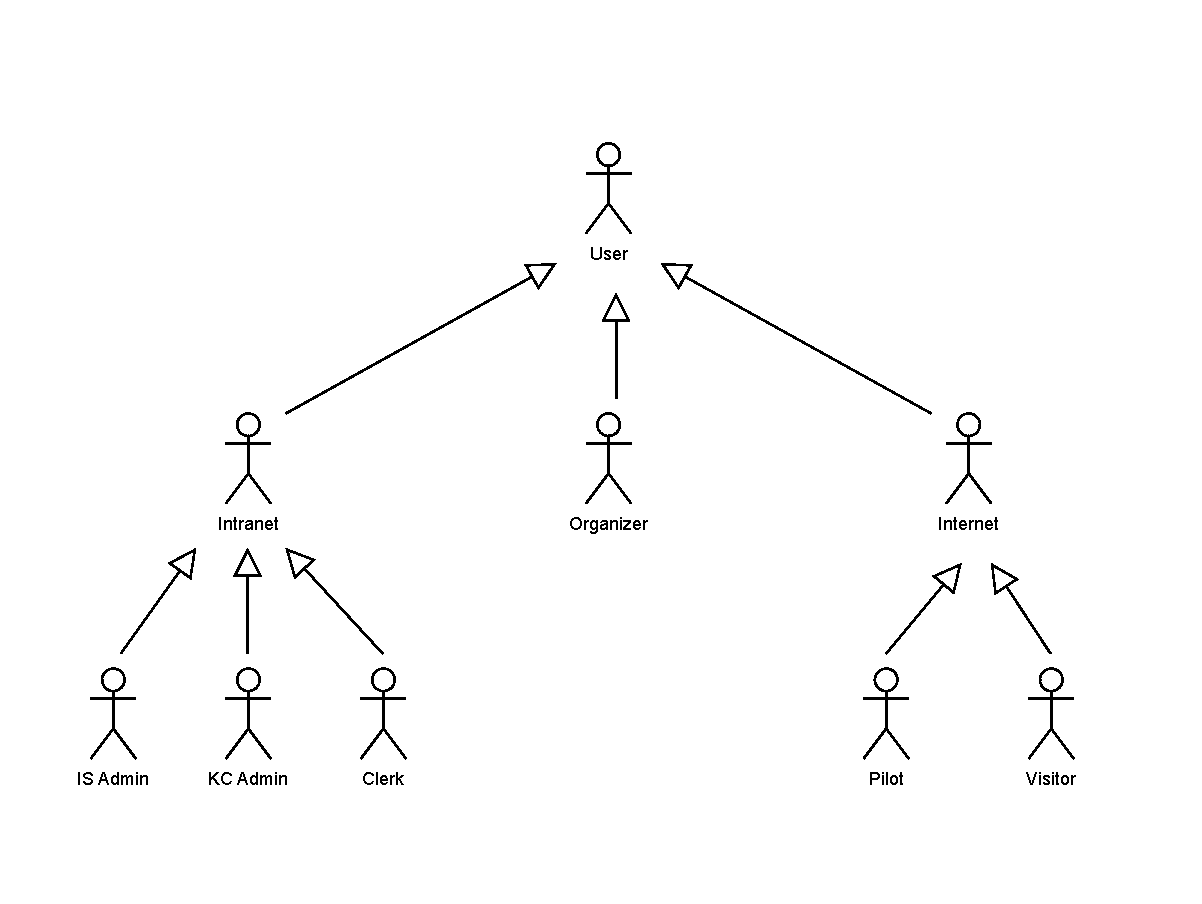
\includegraphics[width=0.8\linewidth]{drawio/users-uc.pdf}
    % \caption{User groups}
\end{figure}
\end{frame}

\begin{frame}
    \frametitle{Specification sheet}
    \begin{table}
        \tiny
        \begin{tabular}{|p{2cm}|p{6cm}|}
        \hline
        Group name & \textbf{Information System Administrator} \\
        \hline
        Description & Empty \\
        \hline
        Profile data & Username, Password, Email, Name, Surname, Address \\
        Supergroup & Intranet \\
        \hline
        Subgroups & None \\
        \hline
        Use cases & 
        - Explore karting center administrators \newline
        - Read details on karting center administrator \newline
        - U.D. karting center administrator \newline
        - Create karting center administrator \newline
        - Explore karting centers \newline
        - Read details on karting center \newline
        - U.D. karting center \newline
        - Create karting center \newline
        - Explore organizers \newline
        - Read details on organizer \newline
        - U.D. organizer \newline
        - Create organizer \newline
        - C.R.U.D. cities \newline
        - C.R.U.D. go-kart models \newline
        - C.R.U.D. track asphalt types \newline
        - C.R.U.D. track length ranges \newline
        - C.R.U.D. review score ranges \newline
        - C.R.U.D. n. pilots ranges \newline
        - C.R.U.D. n. races ranges \newline
        - C.R.U.D. n. events ranges \newline
        - C.R.U.D. price ranges \newline
        - C.R.U.D. event categories \\
        \hline
        \end{tabular}
    \end{table}
\end{frame}
% continue table
\begin{frame}
    \begin{table}
        \tiny
        \begin{tabular}{|p{2cm}|p{6cm}|}
        \hline
        Read & Everything \\
        \hline
        Write & Karting center, Karting center administrator, Organizer, City, Go-kart model, Track asphalt type, Track length range, Review score range, N. pilots range,
        N. races range, N. events range, Price range, Event category, everything that every karting center administrator can write (thus, also everything that every clerk can write) and 
        everything that every organizer can write. \\
        \hline
        \end{tabular}
    \end{table}
\end{frame}

\begin{frame}
\frametitle{Specification sheet}
\begin{table}
    \tiny
    \begin{tabular}{|p{2cm}|p{6cm}|}
    \hline
    Group name & \textbf{Karting center administrator} \\
    \hline
    Description & Empty \\
    \hline
    Profile data & Username, Password, Email, Name, Surname, Address \\
    Supergroup & Intranet \\
    \hline
    Subgroups & None \\
    \hline
    Use cases & 
    - Explore my karting centers \newline
    - Explore pilots by karting center \newline
    - Read details on pilot \newline
    - U.D. pilot \newline
    - Create pilot \newline
    - Explore clerks by karting center \newline
    - Read details on clerk \newline
    - U.D. clerk \newline
    - Create clerk \newline
    - Explore tracks (related to my karting centers)\newline
    - Explore tracks by karting center \newline
    - Read details on track \newline
    - U.D. track \newline
    - Create track \newline
    - Explore races (related to my karting centers) \newline
    - Read details on race \newline
    - U.D. race \newline
    - Create race \newline
    - Explore go-karts dedicated to tracks of my karting centers \newline
    - U.D. go-kart dedicated to track \newline
    - Create go-kart \\
    \hline
    \end{tabular}
\end{table}
\end{frame}
% continue table
\begin{frame}
    \begin{table}
        \tiny
        \begin{tabular}{|p{2cm}|p{6cm}|}
        \hline
        Read & Clerks (related to my karting centers), go-karts (related to my karting centers), everything that every clerk of my karting centers can read,
        everything that the generic user can read. \\
        \hline
        Write & Karting center (only mine, only to update, not to create nor delete), Clerk (only mine), Track (only mine), Race (only for my karting centers), Go-kart (only for my karting centers),
        everything that every clerk of my karting centers can write. \\
        \hline
        \end{tabular}
    \end{table}
\end{frame}





\section*{Use cases}

\subsection*{User}

\begin{frame}
    \frametitle{User}
    \centering
    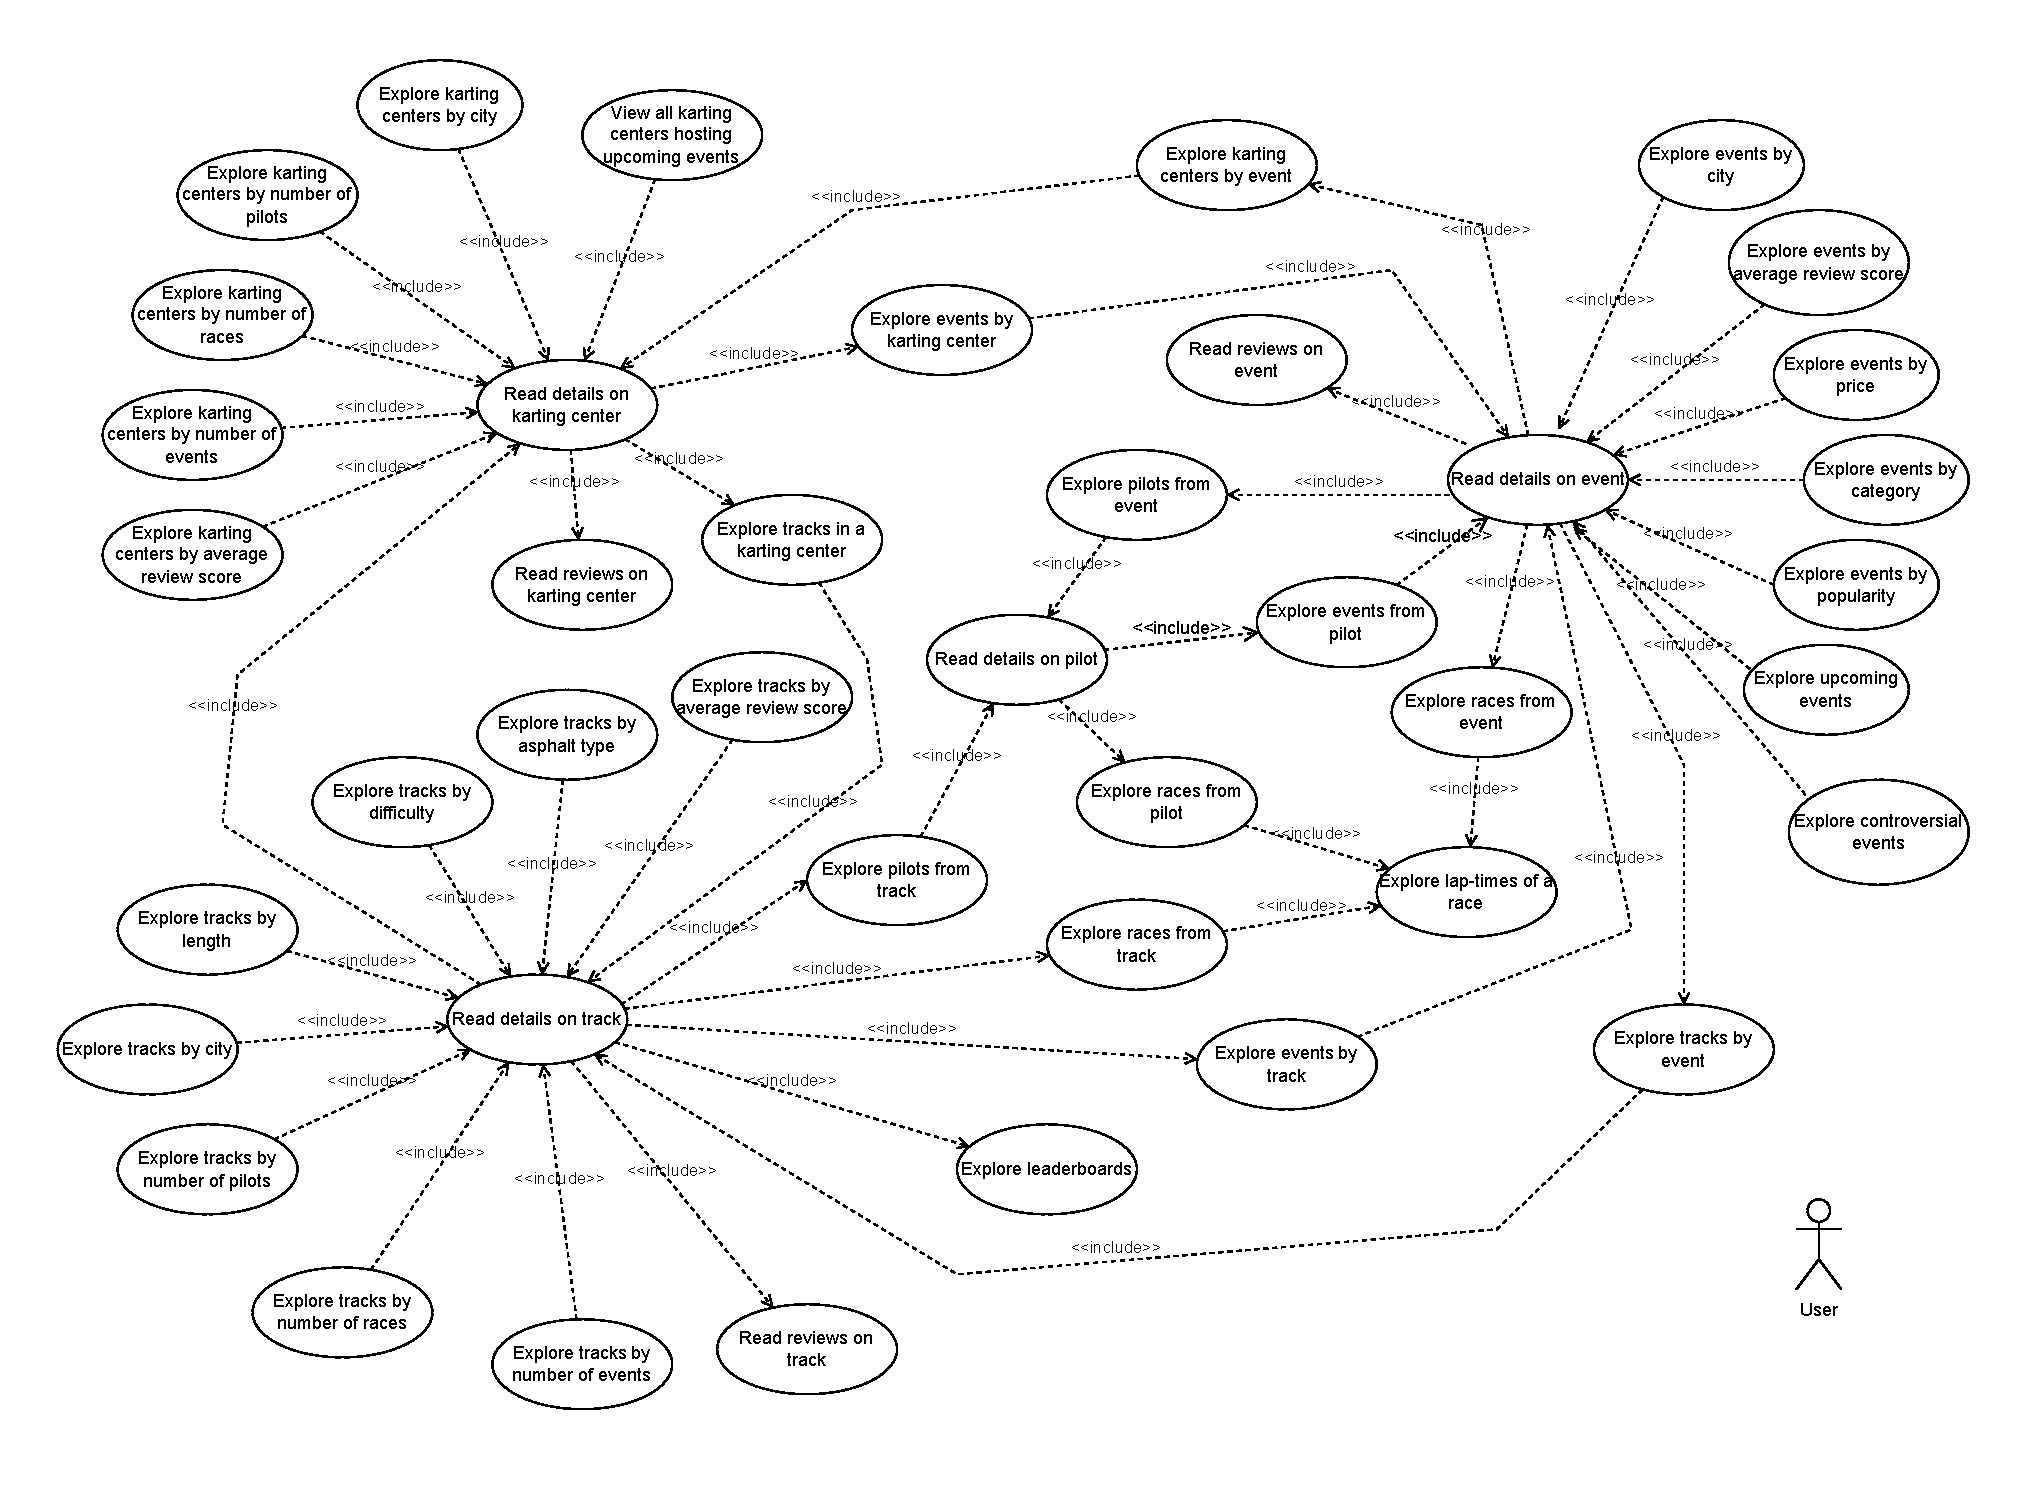
\includegraphics[width=0.8\linewidth]{drawio/user.pdf}
\end{frame}

% %%%%%%%%%% KARTING CENTER AREA %%%%%%%%%%%%%%%

\begin{frame}
\frametitle{Specification sheet}
\begin{table}
    \tiny
    \begin{tabular}{|p{2cm}|p{6cm}|}
    \hline
    Title & \textbf{Explore karting centers by city} \\
    \hline
    Goal & The user seeks karting centers selecting one city at a time. \\
    \hline
    Precondition & The user is in the area (of the public view) dedicated to karting centers.\\
    \hline
    Postcondition & The user obtains the list of karting centers from which he can move on.\\
    \hline
    Workflow &
    - The user moves to the area dedicated to karting centers. \newline
    - The user selects a city. \\
    \hline
    \end{tabular}
\end{table}
\end{frame}

\begin{frame}
    \frametitle{Specification sheet}
    \begin{table}
        \tiny
        \begin{tabular}{|p{2cm}|p{6cm}|}
        \hline
        Title & \textbf{Explore karting centers by number of races} \\
        \hline
        Goal & The user seeks karting centers selecting one range of number of races (that
        were hosted on any of the tracks of the karting center) at a time. \\
        \hline
        Precondition & The user is in the area (of the public view) dedicated to karting centers.\\
        \hline
        Postcondition & The user obtains the list of karting centers from which he can move on.\\
        \hline
        Workflow &
        - The user moves to the area dedicated to karting centers. \newline
        - The user selects a range of number of races. \\
        \hline
        \end{tabular}
\end{table}
\end{frame}


\begin{frame}
    \frametitle{Specification sheet}
    \begin{table}
        \tiny
        \begin{tabular}{|p{2cm}|p{6cm}|}
        \hline
        Title & \textbf{Explore karting centers by number of pilots} \\
        \hline
        Goal & The user seeks karting centers selecting one range of number of pilots (who had a race on 
        any of the tracks of the karting center) at a time. \\
        \hline
        Precondition & The user is in the area (of the public view) dedicated to karting centers.\\
        \hline
        Postcondition & The user obtains the list of karting centers from which he can move on.\\
        \hline
        Workflow &
        - The user moves to the area dedicated to karting centers. \newline
        - The user selects a range of number of pilots. \\
        \hline
        \end{tabular}
\end{table}
\end{frame}

\begin{frame}
    \frametitle{Specification sheet}
    \begin{table}
        \tiny
        \begin{tabular}{|p{2cm}|p{6cm}|}
        \hline
        Title & \textbf{Explore karting centers by number of events} \\
        \hline
        Goal & The user seeks karting centers selecting one range of number of events (that had
        at least one race hosted on 
        any of the tracks of the karting center) at a time. \\
        \hline
        Precondition & The user is in the area (of the public view) dedicated to karting centers.\\
        \hline
        Postcondition & The user obtains the list of karting centers from which he can move on.\\
        \hline
        Workflow &
        - The user moves to the area dedicated to karting centers. \newline
        - The user selects a range of number of events. \\
        \hline
        \end{tabular}
\end{table}
\end{frame}

\begin{frame}
    \frametitle{Specification sheet}
    \begin{table}
        \tiny
        \begin{tabular}{|p{2cm}|p{6cm}|}
        \hline
        Title & \textbf{Explore karting centers by average review score} \\
        \hline
        Goal & The user seeks karting centers selecting one range of average review scores (given to the karting center by all the pilots
        that had at least one race on one of the tracks of the karting center) at a time. \\
        \hline
        Precondition & The user is in the area (of the public view) dedicated to karting centers.\\
        \hline
        Postcondition & The user obtains the list of karting centers from which he can move on.\\
        \hline
        Workflow &
        - The user moves to the area dedicated to karting centers. \newline
        - The user selects a range of scores (the ranges are the same for karting centes, tracks and events). \\
        \hline
        \end{tabular}
\end{table}
\end{frame}

\begin{frame}
    \frametitle{Specification sheet}
    \begin{table}
        \tiny
        \begin{tabular}{|p{2cm}|p{6cm}|}
        \hline
        Title & \textbf{View all karting centers hosting upcoming events} \\
        \hline
        Goal & The user scrolls through the list of karting centers that are going to host an upcoming event. \\
        \hline
        Precondition & The user already has this information in the homepage.\\
        \hline
        Postcondition & The user obtains the list of karting centers from which he can move on.\\
        \hline
        Workflow &
        - The user reaches the homepage. \\
        \hline
        \end{tabular}
\end{table}
\end{frame}

\begin{frame}
    \frametitle{Specification sheet}
    \begin{table}
        \tiny
        \begin{tabular}{|p{2cm}|p{6cm}|}
        \hline
        Title & \textbf{Read details on karting center} \\
        \hline
        Goal & The user chooses one karting center to focus on and reads its details. \\
        \hline
        Precondition & The user chose a karting center from a list of karting centers (obtained from any of the previous use cases).\\
        \hline
        Postcondition & The user obtains the details on the karting center and can move on to other related informations (e.g. tracks, reviews)\\
        \hline
        Workflow &
        - The user chooses one karting center from a list. \\
        \hline
        \end{tabular}
\end{table}
\end{frame}

\begin{frame}
    \frametitle{Specification sheet}
    \begin{table}
        \tiny
        \begin{tabular}{|p{2cm}|p{6cm}|}
        \hline
        Title & \textbf{Read reviews on karting center} \\
        \hline
        Goal & The user chooses one karting center to focus on and scrolls the reviews it received (from pilots
        that had at least one race on one track of the karting center). \\
        \hline
        Precondition & The user chose a karting center from a list of karting centers (obtained from any of the previous use cases).\\
        \hline
        Postcondition & The user obtains the reviews on the karting center in the area dedicated to reviews. \\
        \hline
        Workflow &
        - The user moves from the page dedicated to the details of the karting center to the
        page dedicated to reviews through a click. \\
        \hline
        \end{tabular}
\end{table}
\end{frame}

\begin{frame}
    \frametitle{Specification sheet}
    \begin{table}
        \tiny
        \begin{tabular}{|p{2cm}|p{6cm}|}
        \hline
        Title & \textbf{Explore tracks in a karting center} \\
        \hline
        Goal & The user chooses one karting center to focus on and explores the tracks it offers. \\
        \hline
        Precondition & The user chose a karting center from a list of karting centers (obtained from any of the previous use cases).\\
        \hline
        Postcondition & The user obtains the tracks offered by the karting center in the area dedicated to tracks. \\
        \hline
        Workflow &
        - The user moves from the page dedicated to the details of the karting center to the
        page dedicated to tracks through a click. \\
        \hline
        \end{tabular}
\end{table}
\end{frame}

\begin{frame}
    \frametitle{Specification sheet}
    \begin{table}
        \tiny
        \begin{tabular}{|p{2cm}|p{6cm}|}
        \hline
        Title & \textbf{Explore tracks by asphalt type} \\
        \hline
        Goal & The user seeks tracks selecting one asphalt type at a time. \\
        \hline
        Precondition & The user is in the area (of the public view) dedicated to tracks.\\
        \hline
        Postcondition & The user obtains the list of tracks from which he can move on.\\
        \hline
        Workflow &
        - The user moves to the area dedicated to tracks. \newline
        - The user selects an asphalt type. \\
        \hline
        \end{tabular}
\end{table}
\end{frame}

\begin{frame}
    \frametitle{Specification sheet}
    \begin{table}
        \tiny
        \begin{tabular}{|p{2cm}|p{6cm}|}
        \hline
        Title & \textbf{Explore tracks by difficulty} \\
        \hline
        Goal & The user seeks tracks selecting one difficulty at a time. \\
        \hline
        Precondition & The user is in the area (of the public view) dedicated to tracks.\\
        \hline
        Postcondition & The user obtains the list of tracks from which he can move on.\\
        \hline
        Workflow &
        - The user moves to the area dedicated to tracks. \newline
        - The user selects a difficulty. \\
        \hline
        \end{tabular}
\end{table}
\end{frame}

\begin{frame}
    \frametitle{Specification sheet}
    \begin{table}
        \tiny
        \begin{tabular}{|p{2cm}|p{6cm}|}
        \hline
        Title & \textbf{Explore tracks by length} \\
        \hline
        Goal & The user seeks tracks selecting one range of lengths at a time. \\
        \hline
        Precondition & The user is in the area (of the public view) dedicated to tracks.\\
        \hline
        Postcondition & The user obtains the list of tracks from which he can move on.\\
        \hline
        Workflow &
        - The user moves to the area dedicated to tracks. \newline
        - The user selects a range of lengths. \\
        \hline
        \end{tabular}
\end{table}
\end{frame}

\begin{frame}
    \frametitle{Specification sheet}
    \begin{table}
        \tiny
        \begin{tabular}{|p{2cm}|p{6cm}|}
        \hline
        Title & \textbf{Explore tracks by city} \\
        \hline
        Goal & The user seeks tracks selecting one city at a time. \\
        \hline
        Precondition & The user is in the area (of the public view) dedicated to tracks.\\
        \hline
        Postcondition & The user obtains the list of tracks from which he can move on.\\
        \hline
        Workflow &
        - The user moves to the area dedicated to tracks. \newline
        - The user selects a city. \\
        \hline
        \end{tabular}
\end{table}
\end{frame}

\begin{frame}
    \frametitle{Specification sheet}
    \begin{table}
        \tiny
        \begin{tabular}{|p{2cm}|p{6cm}|}
        \hline
        Title & \textbf{Explore tracks by number of races} \\
        \hline
        Goal & The user seeks tracks selecting one range of number of races
        (that took place on the track) at a time. \\ 
        \hline
        Precondition & The user is in the area (of the public view) dedicated to tracks.\\
        \hline
        Postcondition & The user obtains the list of tracks from which he can move on.\\
        \hline
        Workflow &
        - The user moves to the area dedicated to tracks. \newline
        - The user selects a range of number of races. \\
        \hline
        \end{tabular}
\end{table}
\end{frame}

\begin{frame}
    \frametitle{Specification sheet}
    \begin{table}
        \tiny
        \begin{tabular}{|p{2cm}|p{6cm}|}
        \hline
        Title & \textbf{Explore tracks by number of pilots} \\
        \hline
        Goal & The user seeks tracks selecting one range of number of pilots
        (who had a race on the track) at a time. \\
        \hline
        Precondition & The user is in the area (of the public view) dedicated to tracks.\\
        \hline
        Postcondition & The user obtains the list of tracks from which he can move on.\\
        \hline
        Workflow &
        - The user moves to the area dedicated to tracks. \newline
        - The user selects a range of number of pilots. \\
        \hline
        \end{tabular}
\end{table}
\end{frame}


\begin{frame}
    \frametitle{Specification sheet}
    \begin{table}
        \tiny
        \begin{tabular}{|p{2cm}|p{6cm}|}
        \hline
        Title & \textbf{Explore tracks by number of events} \\
        \hline
        Goal & The user seeks tracks selecting one range of number of events
        (that had at least one race hosted on the track) at a time. \\
        \hline
        Precondition & The user is in the area (of the public view) dedicated to tracks.\\
        \hline
        Postcondition & The user obtains the list of tracks from which he can move on.\\
        \hline
        Workflow &
        - The user moves to the area dedicated to tracks. \newline
        - The user selects a range of number of events. \\
        \hline
        \end{tabular}
\end{table}
\end{frame}

\begin{frame}
    \frametitle{Specification sheet}
    \begin{table}
        \tiny
        \begin{tabular}{|p{2cm}|p{6cm}|}
        \hline
        Title & \textbf{Explore tracks by average review score} \\
        \hline
        Goal & The user seeks tracks selecting one range of average review scores (given to the track by all the pilots
        that had at least one race on the track) at a time. \\
        \hline
        Precondition & The user is in the area (of the public view) dedicated to tracks.\\
        \hline
        Postcondition & The user obtains the list of tracks from which he can move on.\\
        \hline
        Workflow &
        - The user moves to the area dedicated to tracks. \newline
        - The user selects a range of scores (the ranges are the same for karting centes, tracks and events). \\
        \hline
        \end{tabular}
\end{table}
\end{frame}

\begin{frame}
    \frametitle{Specification sheet}
    \begin{table}
        \tiny
        \begin{tabular}{|p{2cm}|p{6cm}|}
        \hline
        Title & \textbf{Read details on track} \\
        \hline
        Goal & The user chooses one track to focus on and reads its details. \\
        \hline
        Precondition & The user chose a track from a list of tracks (obtained from any of the previous use cases).\\
        \hline
        Postcondition & The user obtains the details on the track and can move on to other related informations (e.g. pilots, leaderboards, races, reviews)\\
        \hline
        Workflow &
        - The user chooses one karting center from a list. \\
        \hline
        \end{tabular}
\end{table}
\end{frame}

\begin{frame}
    \frametitle{Specification sheet}
    \begin{table}
        \tiny
        \begin{tabular}{|p{2cm}|p{6cm}|}
        \hline
        Title & \textbf{Read reviews on track} \\
        \hline
        Goal & The user chooses one track to focus on and scrolls the reviews it received (from pilots
        that had at least one race on it). \\
        \hline
        Precondition & The user chose a track from a list of tracks (obtained from any of the previous use cases).\\
        \hline
        Postcondition & The user obtains the reviews on the tracks in the area dedicated to reviews. \\
        \hline
        Workflow &
        - The user moves from the area dedicated to the details of the track to the
        area dedicated to reviews through a click. \\
        \hline
        \end{tabular}
\end{table}
\end{frame}

\begin{frame}
    \frametitle{Specification sheet}
    \begin{table}
        \tiny
        \begin{tabular}{|p{2cm}|p{6cm}|}
        \hline
        Title & \textbf{Explore leaderboards} \\
        \hline
        Goal & The user chooses one track to focus on and explores the leaderboards associated
        to the track (leaderboards are filtering on the whole record of laptimes obtained by pilots in a race,
        a leaderboard can focus on the last month, the last year, sex, weight...) \\
        \hline
        Precondition & The user chose a track from a list of tracks (obtained from any of the previous use cases).\\
        \hline
        Postcondition & The user obtains the list of leaderboards in the area dedicated to leaderboards. \\
        \hline
        Workflow &
        - The user moves from the area dedicated to the details of the track to the
        area dedicated to leaderboards through a click. \\
        \hline
        \end{tabular}
\end{table}
\end{frame}

\begin{frame}
    \frametitle{Specification sheet}
    \begin{table}
        \tiny
        \begin{tabular}{|p{2cm}|p{6cm}|}
        \hline
        Title & \textbf{Explore races from track} \\
        \hline
        Goal & The user chooses one track to focus on and explores the races that took place on the track. \\
        \hline
        Precondition & The user chose a track from a list of tracks (obtained from any of the previous use cases).\\
        \hline
        Postcondition & The user obtains the list of races in the area dedicated to races. \\
        \hline
        Workflow &
        - The user moves from the area dedicated to the details of the track to the
        area dedicated to races through a click. \\
        \hline
        \end{tabular}
\end{table}
\end{frame}

\begin{frame}
    \frametitle{Specification sheet}
    \begin{table}
        \tiny
        \begin{tabular}{|p{2cm}|p{6cm}|}
        \hline
        Title & \textbf{Explore lap-times of a race} \\
        \hline
        Goal & The user chooses one race to focus on and reads all the lap-times made by all the pilots 
        that participated to the race.\\
        \hline
        Precondition & The user chose a race from a list of races (obtained from a track, an event or a pilot).\\
        \hline
        Postcondition & The user obtains the list of lap-times in the area dedicated to lap-times. \\
        \hline
        Workflow &
        - The user moves from the area dedicated to the details of the race to the
        area dedicated to lap-times through a click. \\
        \hline
        \end{tabular}
\end{table}
\end{frame}

\begin{frame}
    \frametitle{Specification sheet}
    \begin{table}
        \tiny
        \begin{tabular}{|p{2cm}|p{6cm}|}
        \hline
        Title & \textbf{Explore pilots from track} \\
        \hline
        Goal & The user chooses one track to focus on and explores the pilots that had at least one race on the track. \\
        \hline
        Precondition & The user chose a track from a list of tracks (obtained from any of the previous use cases).\\
        \hline
        Postcondition & The user obtains the list of pilots in the area dedicated to pilots. \\
        \hline
        Workflow &
        - The user moves from the area dedicated to the details of the track to the
        area dedicated to pilots through a click. \\
        \hline
        \end{tabular}
\end{table}
\end{frame}

\begin{frame}
    \frametitle{Specification sheet}
    \begin{table}
        \tiny
        \begin{tabular}{|p{2cm}|p{6cm}|}
        \hline
        Title & \textbf{Read details on pilot} \\
        \hline
        Goal & The user chooses one pilot to focus on and reads its details. \\
        \hline
        Precondition & The user chose a pilot from a list of pilots (obtained from a track, a race, an event).\\
        \hline
        Postcondition & The user obtains the details on the pilot and can move on to other related informations (e.g. races, events). \\
        \hline
        Workflow &
        - The user chooses one pilot from a list. \\
        \hline
        \end{tabular}
\end{table}
\end{frame}

\begin{frame}
    \frametitle{Specification sheet}
    \begin{table}
        \tiny
        \begin{tabular}{|p{2cm}|p{6cm}|}
        \hline
        Title & \textbf{Explore events from pilot} \\
        \hline
        Goal & The user chooses one pilot to focus on and explores the events that the pilot attended. \\
        \hline
        Precondition & The user chose a pilot from a list of pilots (obtained from a track, a race, an event).\\
        \hline
        Postcondition & The user obtains a list of events in the area dedicated to events. \\
        \hline
        Workflow &
        - The user moves from the area dedicated to the details of the pilot to the
        area dedicated to events through a click. \\
        \hline
        \end{tabular}
\end{table}
\end{frame}

\begin{frame}
    \frametitle{Specification sheet}
    \begin{table}
        \tiny
        \begin{tabular}{|p{2cm}|p{6cm}|}
        \hline
        Title & \textbf{Explore races from pilot} \\
        \hline
        Goal & The user chooses one pilot to focus on and explores the races that the pilot had. \\
        \hline
        Precondition & The user chose a pilot from a list of pilots (obtained from a track, a race, an event).\\
        \hline
        Postcondition & The user obtains a list of races in the area dedicated to races. \\
        \hline
        Workflow &
        - The user moves from the area dedicated to the details of the pilot to the
        area dedicated to races through a click. \\
        \hline
        \end{tabular}
\end{table}
\end{frame}

% EXPLORE EVENTS

\begin{frame}
    \frametitle{Specification sheet}
    \begin{table}
        \tiny
        \begin{tabular}{|p{2cm}|p{6cm}|}
        \hline
        Title & \textbf{Explore events by city} \\
        \hline
        Goal & The user explres events selecting one city at a time. \\
        \hline
        Precondition & The user is in the area (of the public view) dedicated to events.\\
        \hline
        Postcondition & The user obtains the list of events from which he can move on.\\
        \hline
        Workflow &
        - The user moves to the area dedicated to events. \newline
        - The user selects a city. \\
        \hline
        \end{tabular}
\end{table}
\end{frame}


\begin{frame}
    \frametitle{Specification sheet}
    \begin{table}
        \tiny
        \begin{tabular}{|p{2cm}|p{6cm}|}
        \hline
        Title & \textbf{Explore events by average review score} \\
        \hline
        Goal & The user explores events selecting one range of average review scores (given to the event by all the pilots
        that partecipated to it) at a time. \\
        \hline
        Precondition & The user is in the area (of the public view) dedicated to events.\\
        \hline
        Postcondition & The user obtains the list of events from which he can move on.\\
        \hline
        Workflow &
        - The user moves to the area dedicated to events. \newline
        - The user selects a range of scores (the ranges are the same for karting centes, tracks and events). \\
        \hline
        \end{tabular}
\end{table}
\end{frame}

\begin{frame}
    \frametitle{Specification sheet}
    \begin{table}
        \tiny
        \begin{tabular}{|p{2cm}|p{6cm}|}
        \hline
        Title & \textbf{Explore events by price} \\
        \hline
        Goal & The user explores events selecting one range of prices at a time. \\
        \hline
        Precondition & The user is in the area (of the public view) dedicated to events.\\
        \hline
        Postcondition & The user obtains the list of events from which he can move on.\\
        \hline
        Workflow &
        - The user moves to the area dedicated to events. \newline
        - The user selects a range of prices. \\
        \hline
        \end{tabular}
\end{table}
\end{frame}

\begin{frame}
    \frametitle{Specification sheet}
    \begin{table}
        \tiny
        \begin{tabular}{|p{2cm}|p{6cm}|}
        \hline
        Title & \textbf{Explore events by category} \\
        \hline
        Goal & The user explores events selecting one category at a time. \\
        \hline
        Precondition & The user is in the area (of the public view) dedicated to events.\\
        \hline
        Postcondition & The user obtains the list of events from which he can move on.\\
        \hline
        Workflow &
        - The user moves to the area dedicated to events. \newline
        - The user selects a category. \\
        \hline
        \end{tabular}
\end{table}
\end{frame}

\begin{frame}
    \frametitle{Specification sheet}
    \begin{table}
        \tiny
        \begin{tabular}{|p{2cm}|p{6cm}|}
        \hline
        Title & \textbf{Explore events by popularity} \\
        \hline
        Goal & The user explores only the events considered popular (those that have
        at least $N$ partecipants and at least $M$ reviews) \\
        \hline
        Precondition & The user is in the area (of the public view) dedicated to events.\\
        \hline
        Postcondition & The user obtains the list of events from which he can move on.\\
        \hline
        Workflow &
        - The user moves to the area dedicated to events. \newline
        - The user chooses an event from the list of popular events already provided in the area
        dedicated to events. \\
        \hline
        \end{tabular}
\end{table}
\end{frame}

\begin{frame}
    \frametitle{Specification sheet}
    \begin{table}
        \tiny
        \begin{tabular}{|p{2cm}|p{6cm}|}
        \hline
        Title & \textbf{Explore upcoming events} \\
        \hline
        Goal & The user explores only the upcoming events (those whose first race still has to take place). \\
        \hline
        Precondition & The user is in the area (of the public view) dedicated to events or in the homepage (which 
        already shows the list of upcoming events, the list of tracks that will be involved and the list of 
        karting centers that will be involved). \\
        \hline
        Postcondition & The user obtains the list of events from which he can move on.\\
        \hline
        Workflow &
        - A: the user chooses an event from the list of upcoming events already provided in the homepage.\newline
        - B.1: the user moves to the area dedicated to events. \newline
        - B.2: the user chooses an event from the list of upcoming events already provided in the area dedicated
        to events. \\
        \hline
        \end{tabular}
\end{table}
\end{frame}

\begin{frame}
    \frametitle{Specification sheet}
    \begin{table}
        \tiny
        \begin{tabular}{|p{2cm}|p{6cm}|}
        \hline
        Title & \textbf{Explore controversial events} \\
        \hline
        Goal & The user explores only the controversial events (those that have at least $N$ reviews under 25\% of the maximum score
        and at least $M$ reviews over 75\% of the maximum score). \\
        \hline
        Precondition & The user is in the area (of the public view) dedicated to events.\\
        \hline
        Postcondition & The user obtains the list of events from which he can move on.\\
        \hline
        Workflow &
        - The user moves to the area dedicated to events. \newline
        - The user chooses an event from the list of controversial events already provided in the area dedicated to events. \\
        \hline
        \end{tabular}
\end{table}
\end{frame}

\begin{frame}
    \frametitle{Specification sheet}
    \begin{table}
        \tiny
        \begin{tabular}{|p{2cm}|p{6cm}|}
        \hline
        Title & \textbf{Read details on event} \\
        \hline
        Goal & The user chooses one event to focus on and reads its details. \\
        \hline
        Precondition & The user chose an event from a list of events (obtained from any of the previous use cases).\\
        \hline
        Postcondition & The user obtains the details on the event and can move on to other related
        informations (e.g. races, pilots) \\
        \hline
        Workflow &
        - The user chooses one event from a list. \\
        \hline
        \end{tabular}
\end{table}
\end{frame}

\begin{frame}
    \frametitle{Specification sheet}
    \begin{table}
        \tiny
        \begin{tabular}{|p{2cm}|p{6cm}|}
        \hline  
        Title & \textbf{Explore pilots from event} \\
        \hline
        Goal & The user chooses one event to focus on and explores the pilots that partecipated to the event. \\
        \hline
        Precondition & The user chose an event from a list of events (obtained from any of the previous use cases).\\
        \hline
        Postcondition & The user obtains a list of pilots in the area dedicated to pilots. \\
        \hline
        Workflow &
        - The user moves from the area dedicated to the details of the event to the
        area dedicated to pilots through a click. \\
        \hline
        \end{tabular}
\end{table}
\end{frame}

\begin{frame}
    \frametitle{Specification sheet}
    \begin{table}
        \tiny
        \begin{tabular}{|p{2cm}|p{6cm}|}
        \hline  
        Title & \textbf{Read reviews on event} \\
        \hline
        Goal & The user chooses one event to focus on and scrolls the reviews it received (from pilots that 
        participated to the event). \\
        \hline
        Precondition & The user chose an event from a list of events (obtained from any of the previous use cases).\\
        \hline
        Postcondition & The user obtains the reviews on the event in the area dedicated to reviews. \\
        \hline
        Workflow &
        - The user moves from the area dedicated to the details of the event to the
        area dedicated to reviews through a click. \\
        \hline
        \end{tabular}
\end{table}
\end{frame}



% %%%%% EVENT DETAILS, RACES FROM EVENT, PILOTS FROM EVENT, REVIEWS ON EVENT


% 
% 
% 
% 
% INTRANET
% 
% 
% 
% 

\subsection*{Intranet}

\begin{frame}
    \frametitle{Intranet}
    \centering
    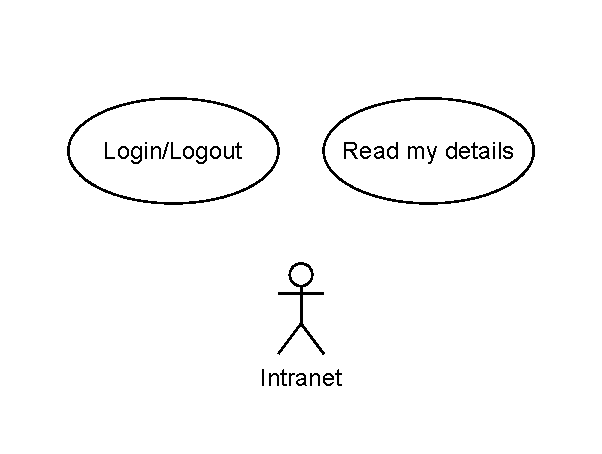
\includegraphics[width=0.7\linewidth]{drawio/intranet.pdf}
\end{frame}

\subsubsection*{Karting center administrator}

\begin{frame}
    \frametitle{Karting center administrator}
    \centering
    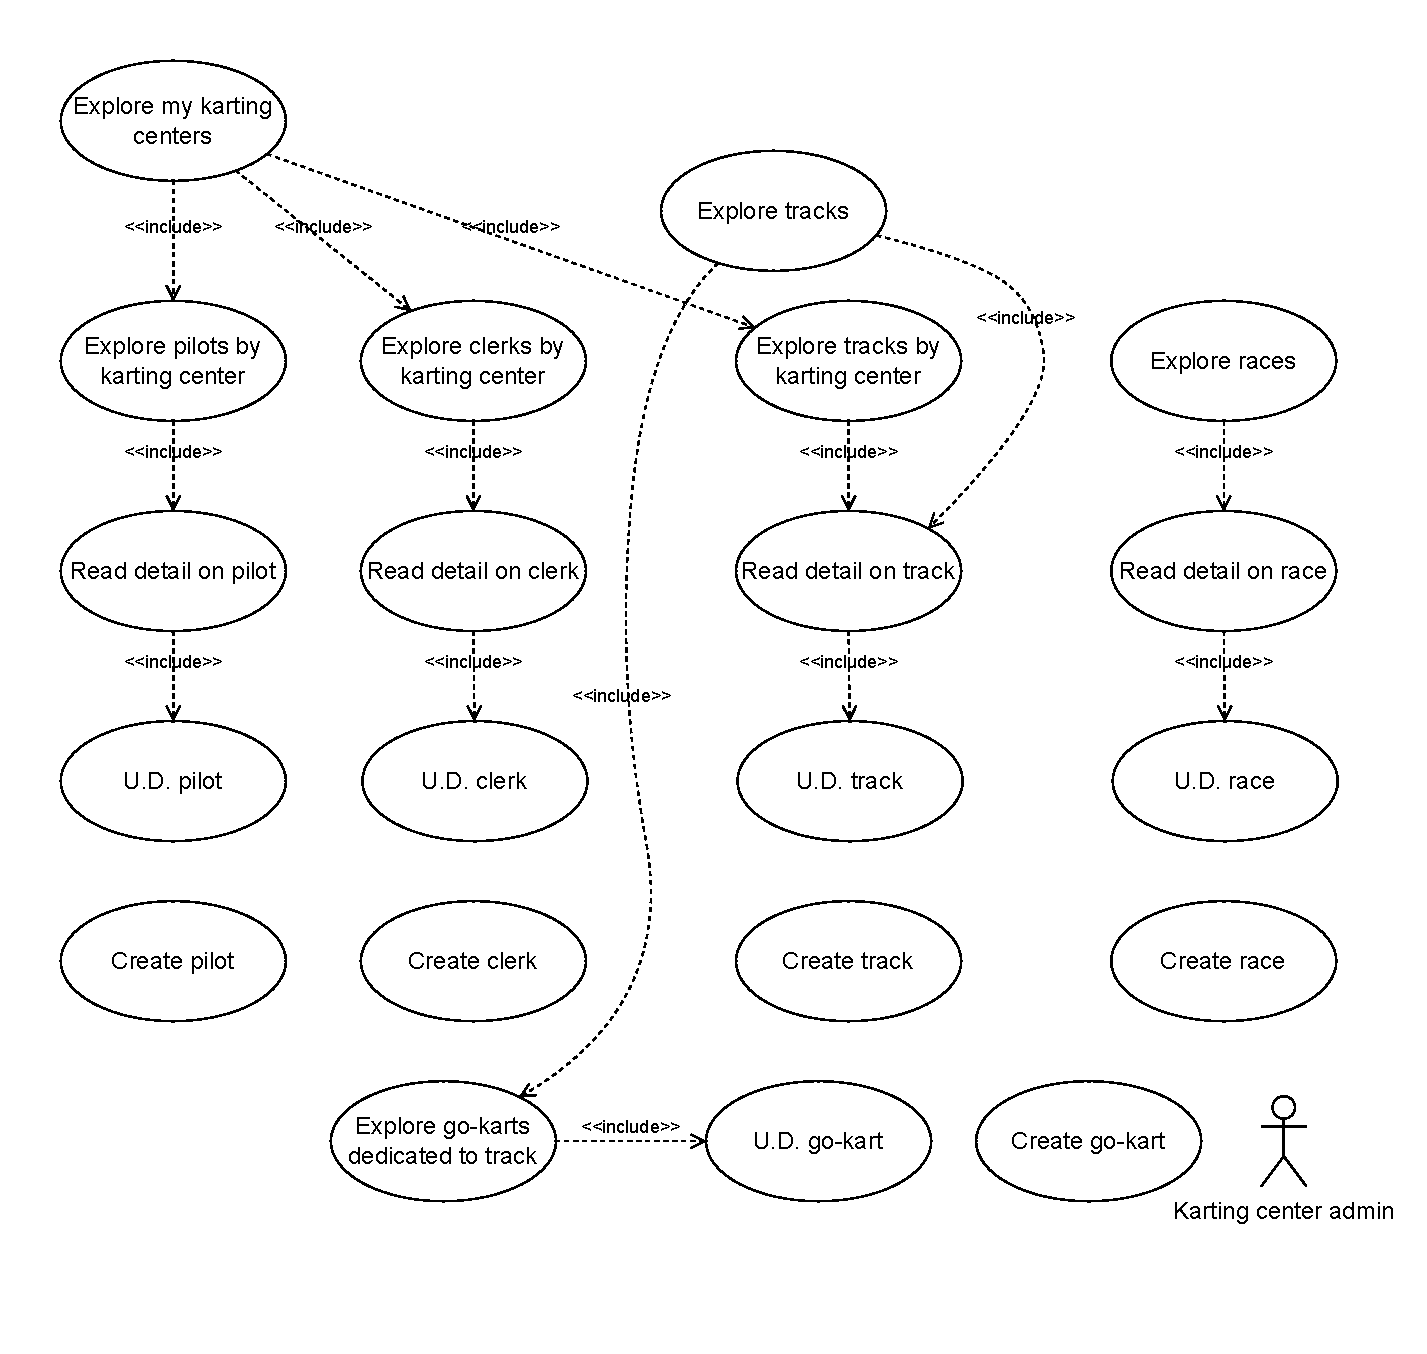
\includegraphics[width=0.7\linewidth]{drawio/karting-center-admin.pdf}
\end{frame}

\begin{frame}
    \frametitle{Specification sheet}
    \begin{table}
        \tiny
        \begin{tabular}{|p{2cm}|p{6cm}|}
        \hline  
        Title & \textbf{Explore my karting centers} \\
        \hline
        Goal & The user explores the karting centers he manages. \\
        \hline
        Precondition & The user logged in and manages at least one karting center.\\
        \hline
        Postcondition & The user obtains the list of karting centers he manages. \\
        \hline
        Workflow &
        - A: the user already has a list of karting centers he manages in the homepage. \newline
        - B: the user moves to the area dedicated to karting centers and the list is already provided. \\
        \hline
        \end{tabular}
\end{table}
\end{frame}

\begin{frame}
    \frametitle{Specification sheet}
    \begin{table}
        \tiny
        \begin{tabular}{|p{2cm}|p{6cm}|}
        \hline  
        Title & \textbf{Explore pilots by karting center} \\
        \hline
        Goal & The user explores the pilots that partecipated in at
        least one race on a track of a karting center the user manages. \\
        \hline
        Precondition & The user logged in, manages at least one karting center and at least one pilot
        had a race on a track of the karting center.\\
        \hline
        Postcondition & The user obtains the list of pilots in the area dedicated to pilots. \\
        \hline
        Workflow &
        - The user chooses the option to explore pilots of a karting center 
        from the list (provided in the homepage) of karting centers he manages. \\
        \hline
        \end{tabular}
\end{table}
\end{frame}


\begin{frame}
    \frametitle{Specification sheet}
    \begin{table}
        \tiny
        \begin{tabular}{|p{2cm}|p{6cm}|}
        \hline  
        Title & \textbf{Explore pilots} \\
        \hline
        Goal & The user explores all the pilots that were registered in any karting center
        by any karting center administrator. \\
        \hline
        Precondition & The user logged in.\\
        \hline
        Postcondition & The user obtains the list of pilots in the area dedicated to pilots. \\
        \hline
        Workflow &
        - The user moves to the area dedicated to pilots (the list is already provided). \\
        \hline
        \end{tabular}
\end{table}
\end{frame}


\begin{frame}
    \frametitle{Specification sheet}
    \begin{table}
        \tiny
        \begin{tabular}{|p{2cm}|p{6cm}|}
        \hline  
        Title & \textbf{Read details on pilot} \\
        \hline
        Goal & The user chooses one pilot to focus on and reads its details. \\
        \hline
        Precondition & The user chose a pilot from a list of pilots (obtained from the homepage,
        from the area dedicated to pilots
        or from the area dedicated to races).\\
        \hline
        Postcondition & The user obtains the details on the pilot (in the area dedicated to pilots). \\
        \hline
        Workflow &
        - The user chooses one pilot from a list (from the homepage, the area dedicated to pilots or 
        the area dedicated to races). \\
        \hline
        \end{tabular}
\end{table}
\end{frame}

\begin{frame}
    \frametitle{Specification sheet}
    \begin{table}
        \tiny
        \begin{tabular}{|p{2cm}|p{6cm}|}
        \hline  
        Title & \textbf{U.D. pilots} \\
        \hline
        Goal & The user updates or deletes a pilot. \\
        \hline
        Precondition & The user logged in. \\
        \hline
        Postcondition & The chosen pilot is updated or deleted. \\
        \hline
        Workflow &
        - The user moves to the area dedicated to pilots. \newline
        - The user chooses the option to update or delete a pilot from 
        the list of all pilots (provided in the area dedicated to pilots). \\
        \hline
        \end{tabular}
\end{table}
\end{frame}


\begin{frame}
    \frametitle{Specification sheet}
    \begin{table}
        \tiny
        \begin{tabular}{|p{2cm}|p{6cm}|}
        \hline  
        Title & \textbf{Create pilots} \\
        \hline
        Goal & The user creates a new pilot. \\
        \hline
        Precondition & The user logged in. \\
        \hline
        Postcondition & The pilot is created. \\
        \hline
        Workflow &
        - The user moves to the area dedicated to pilots. \newline
        - The user chooses the option to create a new pilot. \\
        \hline
        \end{tabular}
\end{table}
\end{frame}

\begin{frame}
    \frametitle{Specification sheet}
    \begin{table}
        \tiny
        \begin{tabular}{|p{2cm}|p{6cm}|}
        \hline  
        Title & \textbf{Explore clerks by karting center} \\
        \hline
        Goal & The user explores the clerks that work in a karting center the user manages. \\
        \hline
        Precondition & The user logged in, manages at least one karting center and at least one clerk
        works in the karting center.\\
        \hline
        Postcondition & The user obtains the list of clerks in the area dedicated to clerks. \\
        \hline
        Workflow &
        - The user chooses the option to explore clerks of a karting center 
        (among the list of karting centers displayed in the homepage) he manages. \\
        \hline
        \end{tabular}
\end{table}

\begin{table}
    \tiny
    \begin{tabular}{|p{2cm}|p{6cm}|}
    \hline  
    Title & \textbf{Explore tracks by karting center} \\
    \hline
    Goal, Precondition, Postcondition, Workflow & Similar to the use case \textbf{Explore clerks by karting center}.
    The user explores the tracks that are part of a karting center the user manages. It is of course
    possible for a karting center administrator to explore all the tracks of all the karting centers
    the same way is is for a visitor, but the site view dedicated to the karting center administrator
    focuses on showing him custom informations. This is not true for the access of the karting center administrator 
    to clerks, he cannot even read informations about clerks from other karting centers, not in his dedicated 
    site view, neither in the visitor's site view.\\
    \hline
    \end{tabular}
\end{table}
\end{frame}


\begin{frame}
    \frametitle{Specification sheet}
    \begin{table}
        \tiny
        \begin{tabular}{|p{2cm}|p{6cm}|}
        \hline  
        Title & \textbf{Explore clerks} \\
        \hline
        Goal & The user explores all the clerks that were registered in any karting center the user manages. \\
        \hline
        Precondition & The user logged in, manages at least one karting center and at least one clerk
        works in the karting center.\\
        \hline
        Postcondition & The user obtains the list of clerks in the area dedicated to clerks. \\
        \hline
        Workflow &
        - The user moves to the area dedicated to clerks (the list is already provided).
        Note: a karting center admin can see all the pilots (also from other karting centers) in the
        area dedicated to pilots but can only see the clerks of the karting centers he manages in the
        area dedicated to clerks. \\
        \hline
        \end{tabular}
\end{table}

\begin{table}
    \tiny
    \begin{tabular}{|p{2cm}|p{6cm}|}
    \hline  
    Title & \textbf{Explore tracks} \\
    \hline
    Goal, Precondition, Postcondition, Workflow & Similar to the use case \textbf{Explore clerks}. \\
    \hline
    \end{tabular}
\end{table}

\begin{table}
    \tiny
    \begin{tabular}{|p{2cm}|p{6cm}|}
    \hline  
    Title & \textbf{Explore races} \\
    \hline
    Goal, Precondition, Postcondition, Workflow & Similar to the use case \textbf{Explore clerks}.
    The user explores all the races that were hosted on any of the tracks in any of the karting centers
    he manages.\\
    \hline
    \end{tabular}
\end{table}
\end{frame}

\begin{frame}
    \frametitle{Specification sheet}
    \begin{table}
        \tiny
        \begin{tabular}{|p{2cm}|p{6cm}|}
        \hline  
        Title & \textbf{Read details on clerk} \\
        \hline
        Goal & The user chooses one clerk to focus on and reads its details. \\
        \hline
        Precondition & The user chose a clerk from a list of clerks (obtained from the homepage,
        from the area dedicated to clerks.)\\
        \hline
        Postcondition & The user obtains the details on the clerk (in the area dedicated to clerks). \\
        \hline
        Workflow &
        - The user chooses one clerk from a list (from the homepage or the area dedicated to clerks). \\
        \hline
        \end{tabular}
\end{table}

\begin{table}
    \tiny
    \begin{tabular}{|p{2cm}|p{6cm}|}
    \hline  
    Title & \textbf{Read details on track} \\
    \hline
    Goal, Precondition, Postcondition, Workflow & Similar to the use case \textbf{Read details on clerk}.\\
    \hline
    \end{tabular}
\end{table}

\begin{table}
    \tiny
    \begin{tabular}{|p{2cm}|p{6cm}|}
    \hline  
    Title & \textbf{Read details on race} \\
    \hline
    Goal, Precondition, Postcondition, Workflow & Similar to the use case \textbf{Read details on clerk}.\\
    \hline
    \end{tabular}
\end{table}
\end{frame}

\begin{frame}
    \frametitle{Specification sheet}
    \begin{table}
        \tiny
        \begin{tabular}{|p{2cm}|p{6cm}|}
        \hline  
        Title & \textbf{U.D. clerks} \\
        \hline
        Goal & The user updates or deletes a clerk. \\
        \hline
        Precondition & The user logged in. \\
        \hline
        Postcondition & The chosen clerk is updated or deleted. \\
        \hline
        Workflow &
        - The user moves to the area dedicated to clerks. \newline
        - The user chooses the option to update or delete a clerk from
        the list of all clerks (provided in the area dedicated to clerks). 
        The user can only update or delete clerks that work for a karting center he manages.\\
        \hline
        \end{tabular}
\end{table}

\begin{table}
    \tiny
    \begin{tabular}{|p{2cm}|p{6cm}|}
    \hline  
    Title & \textbf{U.D. tracks} \\
    \hline
    Goal, Precondition, Postcondition, Workflow & Similar to the use case \textbf{U.D. clerks}.
    The user can update or delete only tracks of karting centers he manages.\\
    \hline
    \end{tabular}
\end{table}

\begin{table}
    \tiny
    \begin{tabular}{|p{2cm}|p{6cm}|}
    \hline  
    Title & \textbf{U.D. races} \\
    \hline
    Goal, Precondition, Postcondition, Workflow & Similar to the use case \textbf{U.D. races}.
    The user can udpdate or delete races that took place or are going to take place on a track 
    of a karting center he manages; when he does, the list of reservations on the same track 
    associated to the race being updated/deleted is shown.\\
    \hline
    \end{tabular}
\end{table}
\end{frame}

\begin{frame}
    \frametitle{Specification sheet}
    \begin{table}
        \tiny
        \begin{tabular}{|p{2cm}|p{6cm}|}
        \hline  
        Title & \textbf{Create clerks} \\
        \hline
        Goal & The user creates a new clerk. \\
        \hline
        Precondition & The user logged in. \\
        \hline
        Postcondition & The clerk is created. \\
        \hline
        Workflow &
        - The user moves to the area dedicated to clerks. \newline
        - The user chooses the option to create a new clerk tht will be visible only to him. \\
        \hline
        \end{tabular}
\end{table}

\begin{table}
    \tiny
    \begin{tabular}{|p{2cm}|p{6cm}|}
    \hline  
    Title & \textbf{Create tracks} \\
    \hline
    Goal, Precondition, Postcondition, Workflow & Similar to the use case \textbf{Create clerks}.
    The track created will be visible to everybody. \\
    \hline
    \end{tabular}
\end{table}

\begin{table}
    \tiny
    \begin{tabular}{|p{2cm}|p{6cm}|}
    \hline  
    Title & \textbf{Create races} \\
    \hline
    Goal, Precondition, Postcondition, Workflow & Similar to the use case \textbf{Create clerks}. 
    When the race is created, an associated reservation (weak entity) is created as well and all the clerks
    working for the karting center that hosts the new race will be able to confirm it.
    The reservation stores the information of the pilot or the organizer that created the race, 
    in this case a fictitious organizer that is created apriori is used.\\
    \hline
    \end{tabular}
\end{table}

\end{frame}


\begin{frame}
    \frametitle{Specification sheet}
    \begin{table}
        \tiny
        \begin{tabular}{|p{2cm}|p{6cm}|}
        \hline  
        Title & \textbf{Explore go-karts dedicated to track (TODO)} \\
        \hline
        Goal & The user explores the go-karts that are dedicated to a track. \\
        \hline
        Precondition & The user logged in, manages at least one karting center that has at least
        one track that has at least one go-kart dedicated to it.\\
        \hline
        Postcondition & The user obtains the list of go-karts in the area dedicated to go-karts. \\
        \hline
        Workflow &
        - A: the user chooses a track from the list of tracks (provided in the homepage) 
        of the karting centers
        he manages. \newline
        - B: the user moves to the area dedicated to tracks and chooses a track from the list of tracks
        (provided in the area dedicated to tracks) of the karting centers he manages. \newline
        - The user chooses the option to explore go-karts dedicated to the track. \\
        \hline
        \end{tabular}
\end{table}
\end{frame}


\begin{frame}
    \frametitle{Specification sheet}
    \begin{table}
        \tiny
        \begin{tabular}{|p{2cm}|p{6cm}|}
        \hline  
        Title & \textbf{U.D. go-karts (TODO)} \\
        \hline
        Goal & The user updates or deletes a go-kart. \\
        \hline
        Precondition & The user logged in and manages at least one karting center that has at least
        one track that has at least one go-kart dedicated to it. \\
        \hline
        Postcondition & The chosen go-kart is updated or deleted. \\
        \hline
        Workflow &
        - A: the user chooses a track from the list of tracks (provided in the homepage) 
        of the karting centers
        he manages. \newline
        - B: the user moves to the area dedicated to tracks and chooses a track from the list of tracks
        (provided in the area dedicated to tracks) of the karting centers he manages. \newline
        - The user chooses the option to update or delete a go-kart from the list of go-karts
        provided in the same page with the details on the track. \\
        \hline
        \end{tabular}
\end{table}
\end{frame}


\begin{frame}
    \frametitle{Specification sheet}
    \begin{table}
        \tiny
        \begin{tabular}{|p{2cm}|p{6cm}|}
        \hline  
        Title & \textbf{Create go-karts (TODO)} \\
        \hline
        Goal & The user creates a new go-kart. \\
        \hline
        Precondition & The user logged in and manages at least one karting center that has at least
        one track. \\
        \hline
        Postcondition & The go-kart is created. \\
        \hline
        Workflow &
        - A: the user chooses a track from the list of tracks (provided in the homepage)
        of the karting centers
        he manages. \newline
        - B: the user moves to the area dedicated to tracks and chooses a track from the list of tracks
        (provided in the area dedicated to tracks) of the karting centers he manages. \newline
        - The user chooses the option to create a new go-kart dedicated to the track 
        from the same page with the details on the track. \\
        \hline
        \end{tabular}
\end{table}
\end{frame}

\subsubsection*{Clerk}

\begin{frame}
    \frametitle{Clerk}
    \centering
    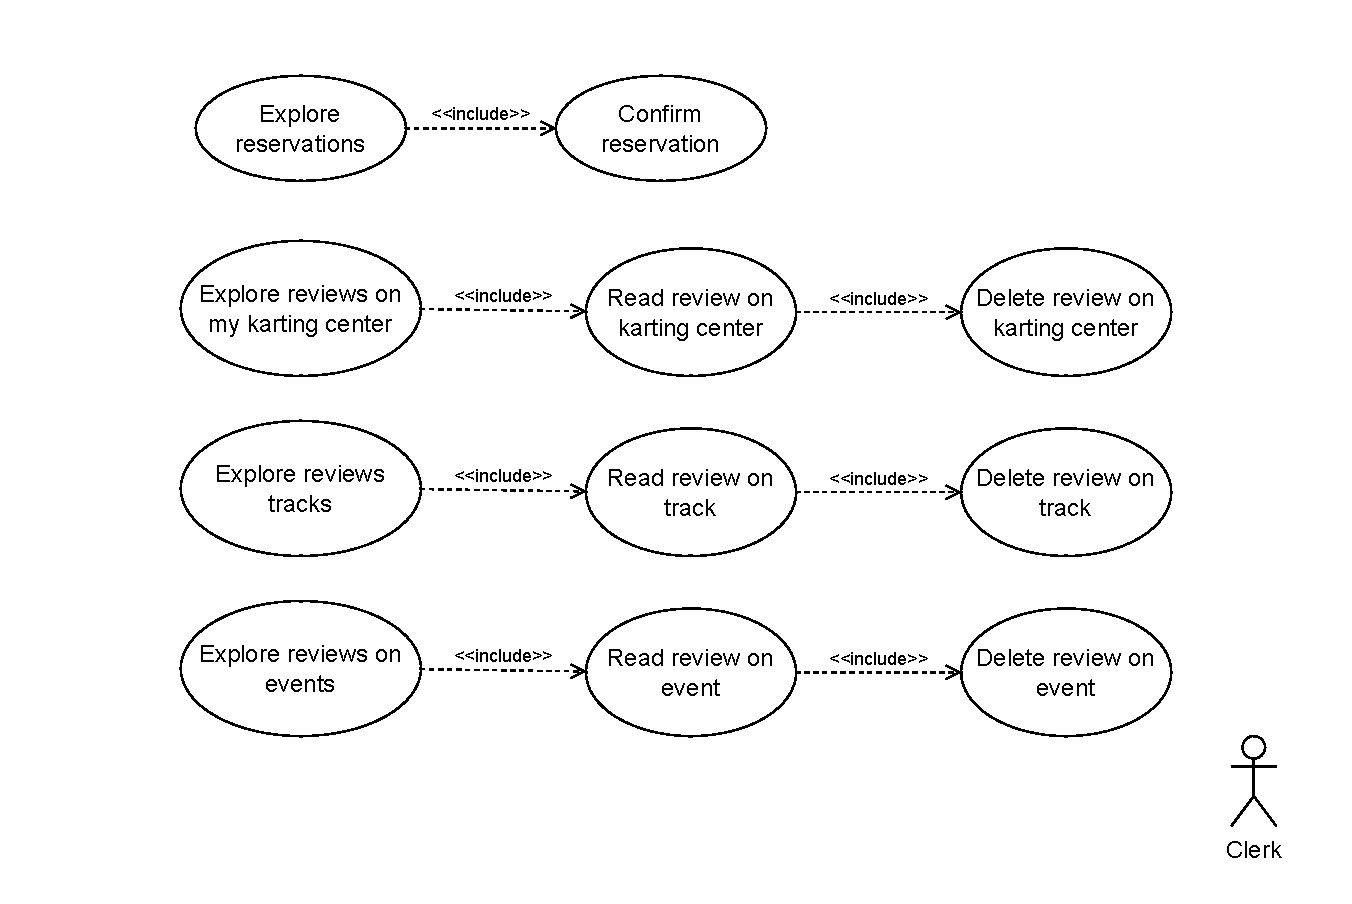
\includegraphics[width=0.9\linewidth]{drawio/clerk.pdf}
\end{frame}

\begin{frame}
    \frametitle{Specification sheet}
    \begin{table}
        \tiny
        \begin{tabular}{|p{2cm}|p{6cm}|}
        \hline  
        Title & \textbf{Explore reservations} \\
        \hline
        Goal & The user explores the reservations asked by pilots on any track of the karting
        center the user works for (a clerk can work on one karting center at a time.) \\
        \hline
        Precondition & The user logged in and works for a karting center
        that received at least a request for reservation on a track. \\
        \hline
        Postcondition & The user obtains the list of reservations in the area dedicated to reservations. \\
        \hline
        Workflow &
        - The user moves to the area dedicated to reservations (a list of the reservations grouped by 
        track is provided). \\
        \hline
        \end{tabular}
\end{table}
\end{frame}


\begin{frame}
    \frametitle{Specification sheet}
    \begin{table}
        \tiny
        \begin{tabular}{|p{2cm}|p{6cm}|}
        \hline  
        Title & \textbf{Confirm reservation} \\
        \hline
        Goal & The user confirms a reservation. \\
        \hline
        Precondition & The user logged in and works for a karting center that received
        at least a request for reservation on a track. \\
        \hline
        Postcondition & The reservation is confirmed (it now has both a pilot/organizer and a clerk associated
        to it). \\
        \hline
        Workflow &
        - The user moves to the area dedicated to reservations. \newline
        - The user chooses the option to confirm a reservation from the list of reservations. \\
        \hline
        \end{tabular}
\end{table}
\end{frame}


\begin{frame}
    \frametitle{Specification sheet}
    \begin{table}
        \tiny
        \begin{tabular}{|p{2cm}|p{6cm}|}
        \hline  
        Title & \textbf{Explore reviews on my karting center} \\
        \hline
        Goal & The user explores the reviews that were written on the karting center the user works for. \\
        \hline
        Precondition & The user logged in and works for a karting center that received
        at least one review. \\
        \hline
        Postcondition & The user obtains the list of reviews on the karting centers. \\
        \hline
        Workflow &
        - The user already has a list of reviews on the karting center he works for in the homepage. \\
        \hline
        \end{tabular}
\end{table}

\begin{table}
    \tiny
    \begin{tabular}{|p{2cm}|p{6cm}|}
    \hline  
    Title & \textbf{Explore reviews on tracks} \\
    \hline
    Goal & The user explores the reviews that were written on tracks of the karting center the user works for. \\
    \hline
    Precondition & The user logged in and works for a karting center that received
    at least one review on a specific track. \\
    \hline
    Postcondition & The user obtains the list of reviews on the tracks. \\
    \hline
    Workflow &
    - The user already has a list of reviews on the karting center he works for in the homepage. \\
    \hline
    \end{tabular}
\end{table}

\begin{table}
    \tiny
    \begin{tabular}{|p{2cm}|p{6cm}|}
    \hline  
    Title & \textbf{Explore reviews on events} \\
    \hline
    Goal & The user explores the reviews that were written on events that hosted at least one race
    on a track of the karting center the user works for. \\
    \hline
    Precondition & The user logged in and works for a karting center that hosted at least one race 
    of an event that received at least one review. \\
    \hline
    Postcondition & The user obtains the list of reviews on the events. \\
    \hline
    Workflow &
    - The user already has a list of reviews on the karting center he works for in the homepage. \\
    \hline
    \end{tabular}
\end{table}

\end{frame}

\begin{frame}
    \frametitle{Specification sheet}
    \begin{table}
        \tiny
        \begin{tabular}{|p{2cm}|p{6cm}|}
        \hline  
        Title & \textbf{Read review on karting center} \\
        \hline
        Goal & The user chooses one review to focus on and reads its details. \\
        \hline
        Precondition & The user logged in and chose a review from the list of reviews on the karting center. \\
        \hline
        Postcondition & The user obtains reads the review and can decide to delete it. \\
        \hline
        Workflow &
        - The user chooses one review from the list of reviews on the karting center (from the homepage). \\
        \hline
        \end{tabular}
    \end{table}

    \begin{table}
        \tiny
        \begin{tabular}{|p{2cm}|p{6cm}|}
        \hline  
        Title & \textbf{Read review on track} \\
        \hline
        Goal, Precondition, Postcondition, Workflow & Similar 
        to the use case \textbf{Read review on karting center}. \\
        \hline
        \end{tabular}
    \end{table}

    \begin{table}
        \tiny
        \begin{tabular}{|p{2cm}|p{6cm}|}
        \hline  
        Title & \textbf{Read review on event} \\
        \hline
        Goal, Precondition, Postcondition, Workflow & Similar 
        to the use case \textbf{Read review on karting center}. \\
        \hline
        \end{tabular}
    \end{table}

\end{frame}

\begin{frame}
    \frametitle{Specification sheet}
    \begin{table}
        \tiny
        \begin{tabular}{|p{2cm}|p{6cm}|}
        \hline  
        Title & \textbf{Delete review on karting center} \\
        \hline
        Goal & The user deletes a review on the karting center. \\
        \hline
        Precondition & The user logged in and chose a review from the list of reviews on the karting center. \\
        \hline
        Postcondition & The user deletes the review. \\
        \hline
        Workflow &
        - The user chooses one review from the list of reviews on the karting center (from the homepage). \newline
        - The user chooses the option to delete the review. \\
        \hline
        \end{tabular}
    \end{table}

    \begin{table}
        \tiny
        \begin{tabular}{|p{2cm}|p{6cm}|}
        \hline  
        Title & \textbf{Delete review on track} \\
        \hline
        Goal, Precondition, Postcondition, Workflow & Similar 
        to the use case \textbf{Delete review on karting center}. \\
        \hline
        \end{tabular}
    \end{table}

    \begin{table}
        \tiny
        \begin{tabular}{|p{2cm}|p{6cm}|}
        \hline  
        Title & \textbf{Delete review on event} \\
        \hline
        Goal, Precondition, Postcondition, Workflow & Similar 
        to the use case \textbf{Delete review on karting center}. \\
        \hline
        \end{tabular}
    \end{table}

\end{frame}

\subsubsection*{Information system administrator}

\begin{frame}
    \frametitle{Information system administrator}
    \centering
    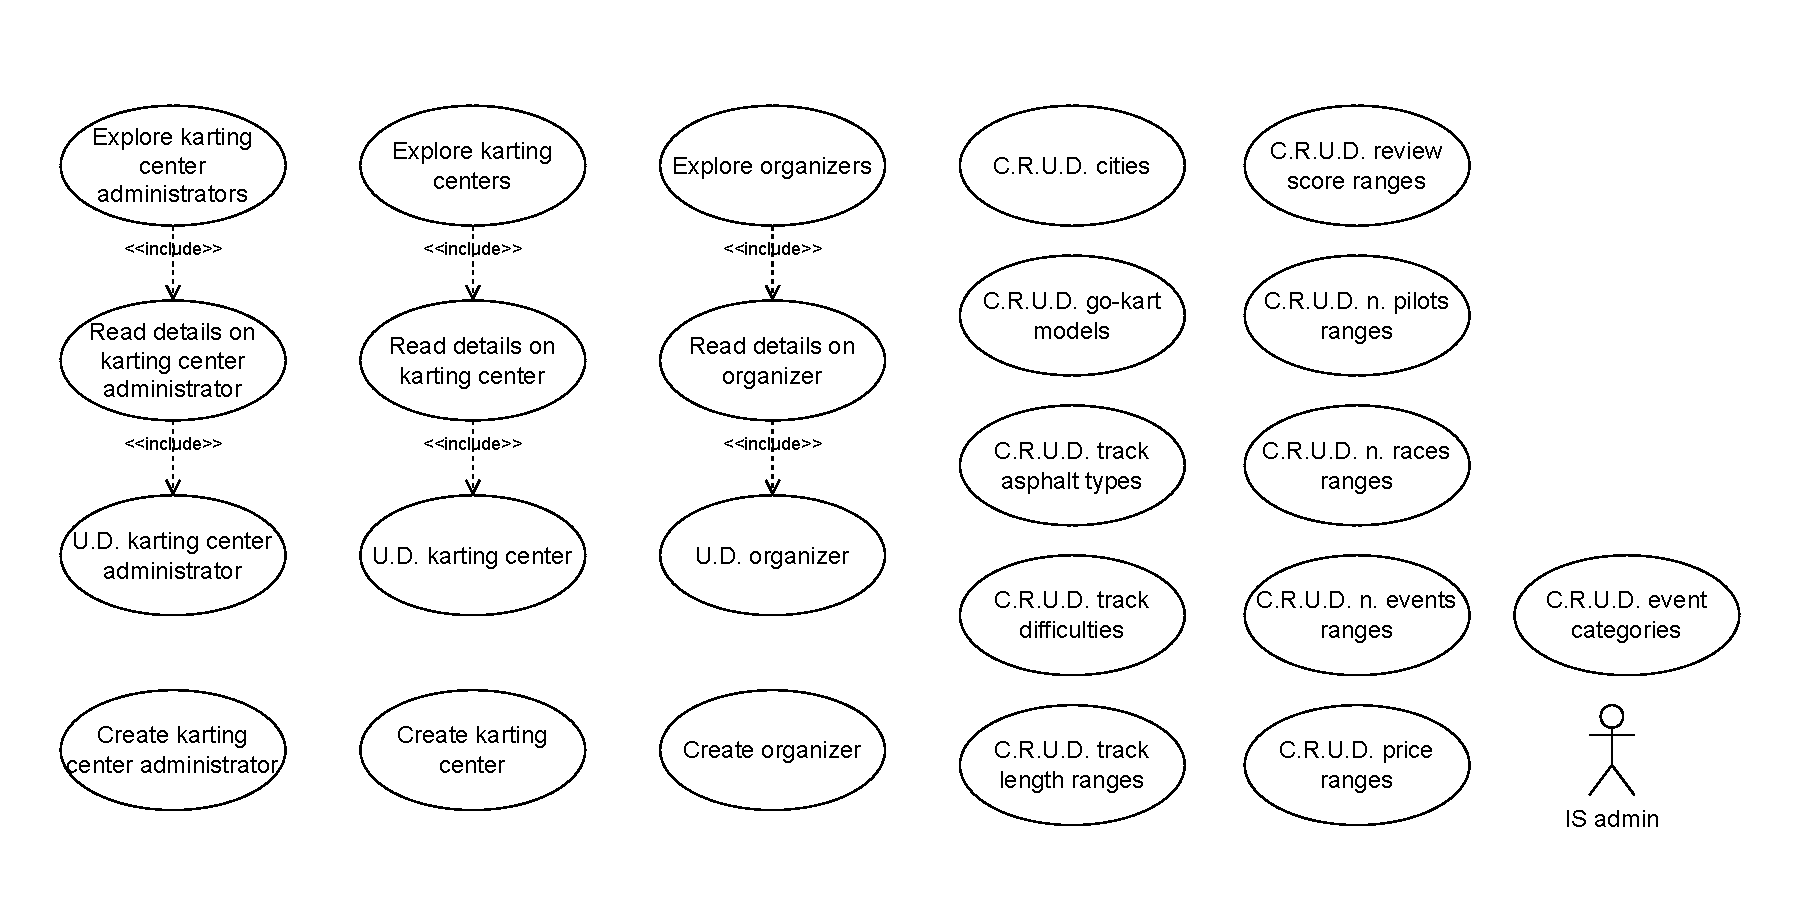
\includegraphics[width=0.7\linewidth]{drawio/is-admin.pdf}
\end{frame}

\begin{frame}
    \frametitle{Specification sheet}
    \begin{table}
        \tiny
        \begin{tabular}{|p{2cm}|p{6cm}|}
        \hline  
        Title & \textbf{Explore karting center administrators} \\
        \hline
        Goal & The user explores the karting center administrators \\
        \hline
        Precondition & The user logged in and has already created at least a karting center 
        administrator. \\
        \hline
        Postcondition & The user obtains the list of karting center administrators. \\
        \hline
        Workflow &
        - The user moves to the area dedicated to karting center administrators. \\
        \hline
        \end{tabular}
\end{table}

\begin{table}
    \tiny
    \begin{tabular}{|p{2cm}|p{6cm}|}
    \hline  
    Title & \textbf{Explore karting centers} \\
    \hline
    Goal, Precondition, Postcondition, Workflow & Similar 
    to the use case \textbf{Explore karting center administrators}. \\
    \hline
    \end{tabular}
\end{table}

\begin{table}
    \tiny
    \begin{tabular}{|p{2cm}|p{6cm}|}
    \hline  
    Title & \textbf{Explore organizers} \\
    \hline
    Goal, Precondition, Postcondition, Workflow & Similar 
    to the use case \textbf{Explore karting center administrators}. \\
    \hline
    \end{tabular}
\end{table}
\end{frame}

\begin{frame}
    \frametitle{Specification sheet}
    \begin{table}
        \tiny
        \begin{tabular}{|p{2cm}|p{6cm}|}
        \hline  
        Title & \textbf{Read details on karting center administrator} \\
        \hline
        Goal & The user chooses one karting center administrator to focus on and reads its details. \\
        \hline
        Precondition & The user logged in and has already created at least a karting center 
        administrator. \\
        \hline
        Postcondition & The user obtains the details on the karting center administrator. \\
        \hline
        Workflow &
        - The user moves to the area dedicated to karting center administrators. \newline
        - The user chooses one karting center administrator from the 
        list of karting center administrators. \\
        \hline
        \end{tabular}
\end{table}

\begin{table}
    \tiny
    \begin{tabular}{|p{2cm}|p{6cm}|}
    \hline  
    Title & \textbf{Read details on karting center} \\
    \hline
    Goal, Precondition, Postcondition, Workflow & Similar 
    to the use case \textbf{Read details on karting center administrator}. \\
    \hline
    \end{tabular}
\end{table}

\begin{table}
    \tiny
    \begin{tabular}{|p{2cm}|p{6cm}|}
    \hline  
    Title & \textbf{Read details on organizer} \\
    \hline
    Goal, Precondition, Postcondition, Workflow & Similar 
    to the use case \textbf{Read details on karting center administrator}. \\
    \hline
    \end{tabular}
\end{table}

\end{frame}

\begin{frame}
    \frametitle{Specification sheet}
    \begin{table}
        \tiny
        \begin{tabular}{|p{2cm}|p{6cm}|}
        \hline  
        Title & \textbf{U.D. karting center administrator} \\
        \hline
        Goal & The user updates or deletes a karting center administrator. \\
        \hline
        Precondition & The user logged in and has already created at least a karting center
        administrator. \\
        \hline
        Postcondition & The chosen karting center administrator is updated or deleted. \\
        \hline
        Workflow &
        - The user moves to the area dedicated to karting center administrators. \newline
        - The user chooses one karting center administrator from the
        list of karting center administrators. \newline
        - The user chooses the option to update or delete the karting center administrator. \\
        \hline
        \end{tabular}
\end{table}

\begin{table}
    \tiny
    \begin{tabular}{|p{2cm}|p{6cm}|}
    \hline  
    Title & \textbf{U.D. karting center} \\
    \hline
    Goal, Precondition, Postcondition, Workflow & Similar 
    to the use case \textbf{U.D. karting center administrator}. \\
    \hline
    \end{tabular}
\end{table}

\begin{table}
    \tiny
    \begin{tabular}{|p{2cm}|p{6cm}|}
    \hline  
    Title & \textbf{U.D. organizer} \\
    \hline
    Goal, Precondition, Postcondition, Workflow & Similar 
    to the use case \textbf{U.D. karting center administrator}. \\
    \hline
    \end{tabular}
\end{table}

\end{frame}

\begin{frame}
    \frametitle{Specification sheet}
    \begin{table}
        \tiny
        \begin{tabular}{|p{2cm}|p{6cm}|}
        \hline  
        Title & \textbf{Create karting center administrator} \\
        \hline  
        Goal & The user creates a new karting center administrator. \\
        \hline
        Precondition & The user logged in. \\
        \hline
        Postcondition & The karting center administrator is created. \\
        \hline
        Workflow &
        - The user moves to the area dedicated to karting center administrators. \newline
        - The user chooses the option to create a new karting center administrator. \\
        \hline
        \end{tabular}
\end{table}

\begin{table}
    \tiny
    \begin{tabular}{|p{2cm}|p{6cm}|}
    \hline  
    Title & \textbf{Create karting center} \\
    \hline
    Goal, Precondition, Postcondition, Workflow & Similar 
    to the use case \textbf{Create karting center administrator}. \\
    \hline
    \end{tabular}
\end{table}

\begin{table}
    \tiny
    \begin{tabular}{|p{2cm}|p{6cm}|}
    \hline  
        Title & \textbf{Create organizer} \\
        \hline
        Goal, Precondition, Postcondition, Workflow & Similar 
        to the use case \textbf{Create karting center administrator}. \\
        \hline
        \end{tabular}
\end{table}

\end{frame}

\begin{frame}
    The karting center administrator is responsible for the management of 
    all those entities useful to the visitors to navigate the site.
    He has the possibility to create, update and delete the following entities:
    \begin{itemize}
        \item City
        \item Go-kart model
        \item Track asphalt type
        \item Track difficulty
        \item Track length range
        \item Review score range
        \item Number of pilots range
        \item Number of races range
        \item Number of events range
        \item Price range
        \item Event category
    \end{itemize} 
\end{frame}

\subsection*{Extranet}

\subsubsection*{Pilot}

\begin{frame}
    \frametitle{Organizer}
    \centering
    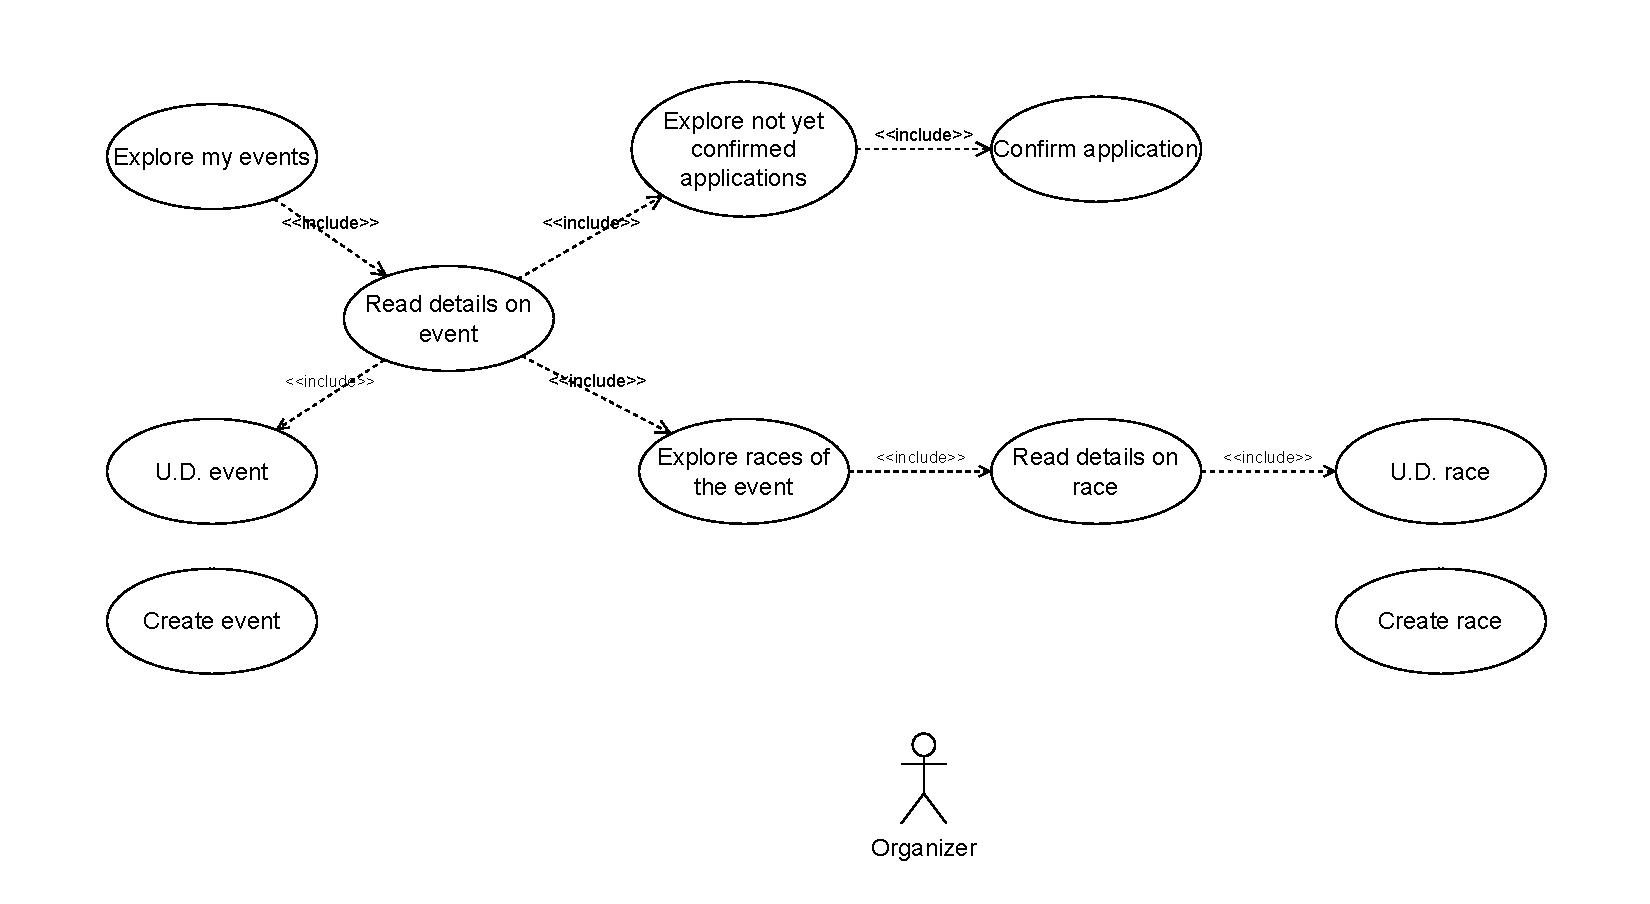
\includegraphics[width=0.9\linewidth]{drawio/organizer.pdf}
\end{frame}


\begin{frame}
    \frametitle{Specification sheet}
    \begin{table}
        \tiny
        \begin{tabular}{|p{2cm}|p{6cm}|}
        \hline
        Title & \textbf{Explore my events} \\
        \hline
        Goal & The user explores the events he created. \\
        \hline
        Precondition & The user logged in and created at least one event.\\
        \hline
        Postcondition & The user obtains the list of events he created. \\
        \hline
        Workflow &
        - A: the user already has a list of events he created and the applications received for each event 
        in the homepage. \newline
        - B: the user moves to the area dedicated to events and the list is already provided. \\
        \hline
        \end{tabular}
\end{table}
\end{frame}


\begin{frame}
    \frametitle{Specification sheet}
    \begin{table}
        \tiny
        \begin{tabular}{|p{2cm}|p{6cm}|}
        \hline
        Title & \textbf{Read details on my event} \\
        \hline
        Goal & The user chooses one event to focus on and reads its details. \\
        \hline
        Precondition & The user logged in. \\
        \hline
        Postcondition & The user obtains the details on the event and 
        can move on to other related informations (e.g. applications). \\
        \hline
        Workflow &
        - A: the user chooses one event from the list of events he created in the homepage. \newline
        - B.1: the user moves to the area dedicated to events. \newline
        - B.2: the user chooses one event from the list of events he created in the area dedicated to events. \\
        \hline
        \end{tabular}
\end{table}
\end{frame}


\begin{frame}
    \frametitle{Specification sheet}
    \begin{table}
        \tiny
        \begin{tabular}{|p{2cm}|p{6cm}|}
        \hline
        Title & \textbf{U.D. events} \\
        \hline
        Goal & The user updates or deletes an event he created. \\
        \hline
        Precondition & The user logged in and he created at least one event. \\
        \hline
        Postcondition & The event is updated or deleted, the modifications might affect the races created for the track 
        and the participations of the pilots to the races of the event but the applications made by pilots are not affected. \\
        \hline
        Workflow &
        - A: the user chooses one event from the list of events he created in the homepage. \newline
        - B.1: the user moves to the area dedicated to events. \newline
        - B.2: the user chooses one event from the list of events he created in the area dedicated to events. \newline
        - The user chooses the option to update or delete the event. \\
        \hline
        \end{tabular}
\end{table}
\end{frame}


\begin{frame}
    \frametitle{Specification sheet}
    \begin{table}
        \tiny
        \begin{tabular}{|p{2cm}|p{6cm}|}
        \hline
        Title & \textbf{Create event} \\
        \hline
        Goal & The user creates a new event. \\
        \hline
        Precondition & The user logged in and created at least one race.\\
        \hline
        Postcondition & The event is created and pilots can apply to it. \\
        \hline
        Workflow &
        - The user moves to the area dedicated to events. \newline
        - The user chooses the option to create a new event (he will need to choose among races he created
        to fill the event). \\
        \hline
        \end{tabular}
\end{table}
\end{frame}

\begin{frame}
    \frametitle{Specification sheet}
    \begin{table}
        \tiny
        \begin{tabular}{|p{2cm}|p{6cm}|}
        \hline
        Title & \textbf{Explore not yet confirmed applications} \\
        \hline
        Goal & The user explores the applications received for his events that he did not confirm yet. \\
        \hline
        Precondition & The user logged in, created at least one event and at least one pilot applied to it.\\
        \hline
        Postcondition & The user obtains the list of applications that he did not confirm yet. \\
        \hline
        Workflow &
        - A: the user chooses one event from the list of events he created in the homepage. \newline
        - B.1: the user moves to the area dedicated to events. \newline
        - B.2: the user chooses one event from the list of events he created in the area dedicated to events. \newline
        (- The list of applications not yet confirmed is already provided.) \\
        \hline
        \end{tabular}
\end{table}
\end{frame}


% \begin{frame}
%     \frametitle{Specification sheet}
%     \begin{table}
%         \tiny
%         \begin{tabular}{|p{2cm}|p{6cm}|}
%         \hline
%         Title & \textbf{Explore not yet confirmed applications} \\
%         \hline
%         Goal & The user explores the applications received for his events that he did not confirm yet. \\
%         \hline
%         Precondition & The user logged in, created at least one event and at least one pilot applied to it.\\
%         \hline
%         Postcondition & The user obtains the list of applications that he did not confirm yet. \\
%         \hline
%         Workflow &
%         - The user follows the same steps as in the use case \textbf{Read details on my event}
%         and the list of applications not yet confirmed is already provided. \\
%         \hline
%         \end{tabular}
% \end{table}
% \end{frame}


\begin{frame}
    \frametitle{Specification sheet}
    \begin{table}
        \tiny
        \begin{tabular}{|p{2cm}|p{6cm}|}
        \hline
        Title & \textbf{Confirm application} \\
        \hline
        Goal & The user confirms an application received for one of his events. \\
        \hline
        Precondition & The user logged in, created at least one event and at least one pilot applied to it.\\
        \hline
        Postcondition & The application is confirmed and the pilot is automatically inserted as a partecipant
        to all of the races of the event (this might change, e.g. in case the organizer decides to organize races 
        in a tournament fashion, but the application will not be affected). \\
        \hline
        Workflow &
        - A: the user chooses one event from the list of events he created in the homepage. \newline
        - B.1: the user moves to the area dedicated to events. \newline
        - B.2: the user chooses one event from the list of events he created in the area dedicated to events. \newline
        - The user chooses the option to accept an application from the list of applications not yet confirmed. \\
        \hline
        \end{tabular}
\end{table}
\end{frame}

\begin{frame}
    \frametitle{Specification sheet}
    \begin{table}
        \tiny
        \begin{tabular}{|p{2cm}|p{6cm}|}
        \hline
        Title & \textbf{Explore races of the event} \\
        \hline
        Precondition & The user logged in, created at least one event and the event has at least one race. \\
        \hline
        Postcondition & The user obtains the list of races of a specific event. \\
        \hline
        Workflow &
        - A: the user chooses one event from the list of events he created in the homepage. \newline
        - B.1: the user moves to the area dedicated to events. \newline
        - B.2: the user chooses one event from the list of events he created in the area dedicated to events. \newline
        (- The list of races of the chosen event is already provided.) \\
        \hline
        \end{tabular}
\end{table}
\end{frame}

\begin{frame}
    \frametitle{Specification sheet}
    \begin{table}
        \tiny
        \begin{tabular}{|p{2cm}|p{6cm}|}
        \hline
        Title & \textbf{Read details on race} \\
        \hline
        Precondition & The user logged in, created at least one event and the event has at least one race. \\
        \hline
        Postcondition & The user obtains the details on the race and can move on (e.g. updating or deleting it.) \\
        \hline
        Workflow &
        - A: the user chooses one event from the list of events he created in the homepage. \newline
        - B.1: the user moves to the area dedicated to events. \newline
        - B.2: the user chooses one event from the list of events he created in the area dedicated to events. \newline
        - The user chooses one race from the list of races of the chosen event. \\
        \hline
        \end{tabular}
\end{table}
\end{frame}


\begin{frame}
    \frametitle{Specification sheet}
    \begin{table}
        \tiny
        \begin{tabular}{|p{2cm}|p{6cm}|}
        \hline
        Title & \textbf{U.D. race} \\
        \hline
        Precondition & The user logged in, created at least one event and the event has at least one race. \\
        \hline
        Postcondition & The race gets updated or deleted, this affects the relations with the pilots (\textit{partecipation})
        but not the application of the pilots to the event. \\
        \hline
        Workflow &
        - A: the user chooses one event from the list of events he created in the homepage. \newline
        - B.1: the user moves to the area dedicated to events. \newline
        - B.2: the user chooses one event from the list of events he created in the area dedicated to events. \newline
        - The user chooses one race from the list of races of the chosen event. \newline
        - The user chooses the option to update or delete the race. \\
        \hline
        \end{tabular}
\end{table}
\end{frame}

\begin{frame}
    \frametitle{Specification sheet}
    \begin{table}
        \tiny
        \begin{tabular}{|p{2cm}|p{6cm}|}
        \hline
        Title & \textbf{Create race} \\
        \hline
        Precondition & The user logged in. \\
        \hline
        Postcondition & A new race is available to the user to be added to an event. \\
        \hline
        Workflow &
        - The user moves to the area dedicated to events. \newline
        - The user chooses the option to create a new race. \\
        \hline
        \end{tabular}
\end{table}
\end{frame}


\subsection*{Internet}

\subsubsection*{Pilot}

\begin{frame}
    \frametitle{Pilot}
    \centering
    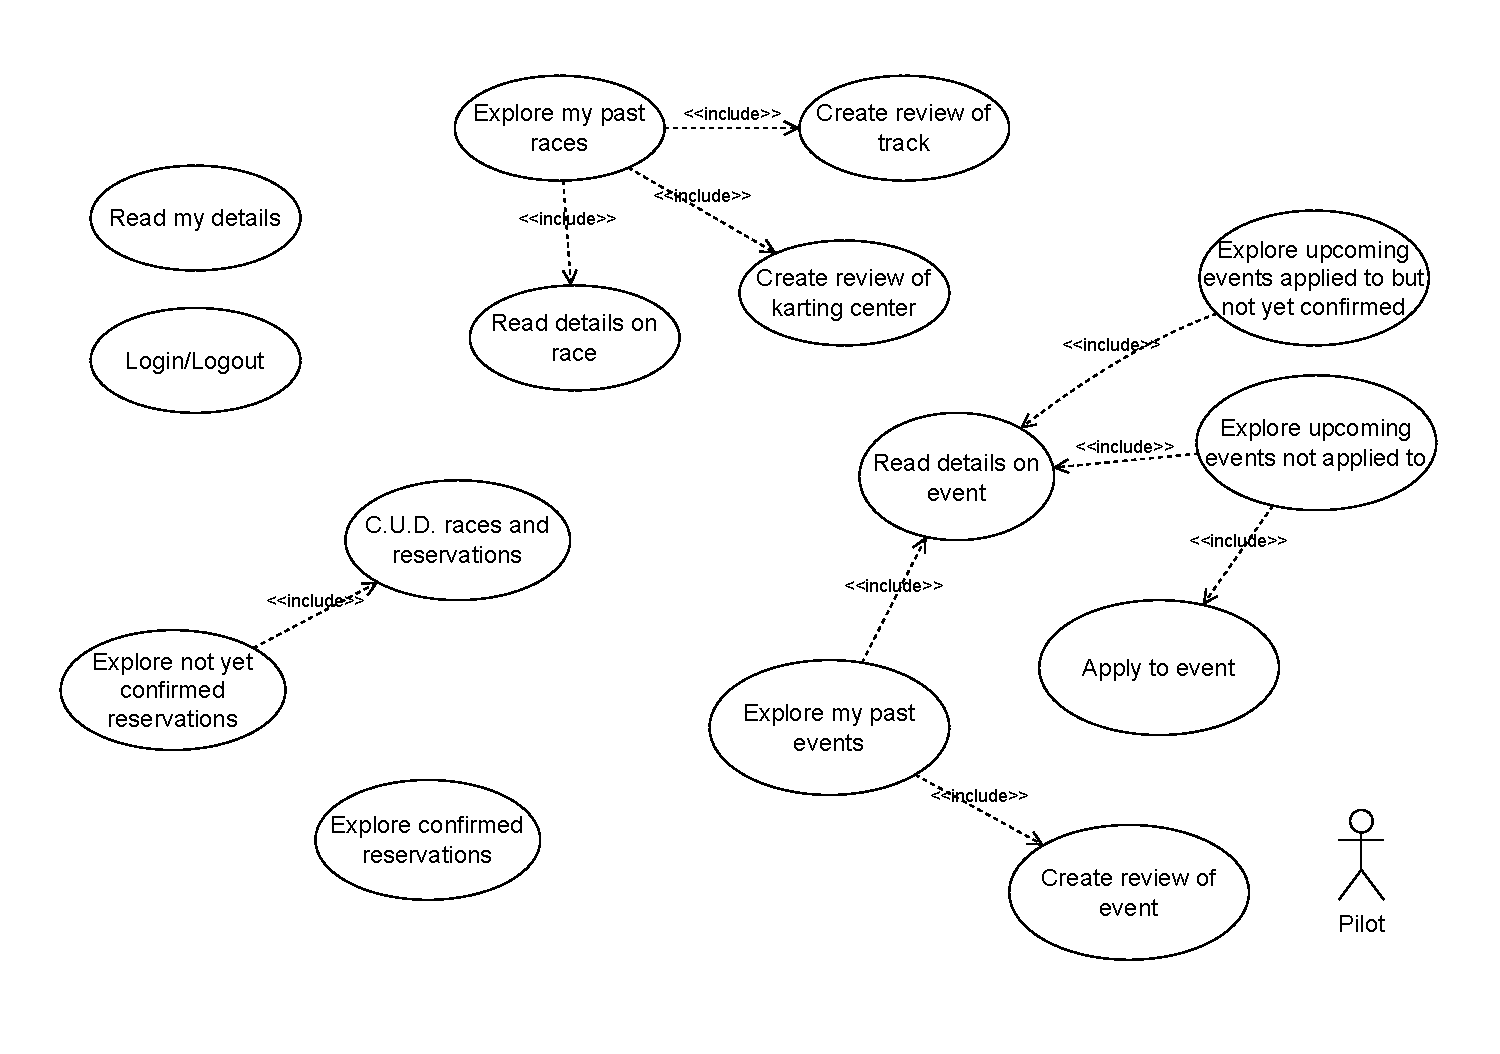
\includegraphics[width=0.9\linewidth]{drawio/pilot.pdf}
\end{frame}

% %%%%% PILOT USE CASE SHEET %%%%%

\begin{frame}
    \frametitle{Specification sheet}
    \begin{table}
        \tiny
        \begin{tabular}{|p{2cm}|p{6cm}|}
        \hline
        Title & \textbf{Read my details} \\
        \hline
        Goal & The user reads its own personal informations, already available in the homepage.\\
        \hline
        Precondition & The user logged in. \\
        \hline
        Postcondition & The user obtains its personal informations. \\
        \hline
        Workflow &
        - The user logs in and reads the informations already present in the homepage. \\
        \hline
        \end{tabular}
\end{table}
\end{frame}

\begin{frame}
    \frametitle{Specification sheet}
    \begin{table}
        \tiny
        \begin{tabular}{|p{2cm}|p{6cm}|}
        \hline
        Title & \textbf{Explore not yet confirmed reservations} \\
        \hline
        Goal & The user explores the reservations he made that are not yet confirmed by any clerk \\
        \hline
        Precondition & The user logged in. \\
        \hline
        Postcondition & The user obtains the list of reservations that are not yet confirmed by any clerk. \\
        \hline
        Workflow &
        - The user moves to the area dedicated to reservations and the list is already provided. \\
        \hline
        \end{tabular}
\end{table}
\end{frame}


\begin{frame}
    \frametitle{Specification sheet}
    \begin{table}
        \tiny
        \begin{tabular}{|p{2cm}|p{6cm}|}
        \hline
        Title & \textbf{C.U.D. races and reservations} \\
        \hline
        Goal & The user asks for a reservation to have a race on a track of a karting center. \\
        \hline
        Precondition & The user logged in. \\
        \hline
        Postcondition & A race and its relative reservation (a weak entity of the race) are created, updated or deleted. \\
        \hline
        Workflow &
        - The user moves to the area dedicated to reservations. \newline
        - A: the user selects a reservation from those not yet confirmed and updates it or deletes it. \newline
        - B: the user creates a new reservation without the need to select one from those not yet confirmed. \newline
        Note: the existence of the reservation is hidden to the user when he creates/updates/deletes the race,
        the reservation just takes some of the attributes of the race (Date, Start, End) and is shared with the clerks
        of the karting center, who can confirm it or not. The user can only see the reservations that are
        confirmed or not, he does not edit them directly but only through the actions on the race. \\
        \hline
        \end{tabular}
\end{table}
\end{frame}


\begin{frame}
    \frametitle{Specification sheet}
    \begin{table}
        \tiny
        \begin{tabular}{|p{2cm}|p{6cm}|}
        \hline
        Title & \textbf{Explore confirmed reservations} \\
        \hline
        Goal & The user explores the reservations he made that are confirmed by a clerk \\
        \hline
        Precondition & The user logged in. \\
        \hline
        Postcondition & The user obtains the list of reservations that are confirmed by a clerk. \\
        \hline
        Workflow &
        - The user moves to the area dedicated to reservations and the list is already provided. \\
        \hline
        \end{tabular}
\end{table}
\end{frame}

\begin{frame}
    \frametitle{Specification sheet}
    \begin{table}
        \tiny
        \begin{tabular}{|p{2cm}|p{6cm}|}
        \hline
        Title & \textbf{Explore my past races} \\
        \hline
        Goal & The user explores the races he had in the past (not the races he booked through the previous 
        use case). \\
        \hline
        Precondition & The user logged in. \\
        \hline  
        Postcondition & The user obtains the list of past races. \\
        \hline
        Workflow &
        - The user moves to the area dedicated to races
        and the list is already provided. \\
        \hline
        \end{tabular}
\end{table}
\end{frame}

\begin{frame}
    \frametitle{Specification sheet}
    \begin{table}
        \tiny
        \begin{tabular}{|p{2cm}|p{6cm}|}
        \hline
        Title & \textbf{Read details on race} \\
        \hline
        Goal & The user chooses one race to focus on and reads its details. \\
        \hline
        Precondition & The user logged in. \\
        \hline
        Postcondition & The user obtains the details on the race and related informations such as the best lap-time of
        that race (it could be from the user himself or another pilot). \\
        \hline
        Workflow &
        - The user moves to the area dedicated to races. \newline
        - The user chooses one race from the list of past races. \\
        \hline
        \end{tabular}
\end{table}
\end{frame}


\begin{frame}
    \frametitle{Specification sheet}
    \begin{table}
        \tiny
        \begin{tabular}{|p{2cm}|p{6cm}|}
        \hline
        Title & \textbf{Create review of karting center} \\
        \hline
        Goal & The user creates a review of a karting center. \\
        \hline
        Precondition & The user logged in and had at least one race that will allow him to write 
        reviews for the track and the karting center that hosted that race. \\
        \hline
        Postcondition & The review is stored and a clerk of the karting center will be able to 
        read it and remove it if it is considered inappropriate. \\
        \hline
        Workflow &
        - The user moves to the area dedicated to reviews. \newline
        - From the list of past races, the user selects the option to write a review of the karting center that
        hosted the chosen race from the list. \newline
        - The user chooses a score, writes the review and submits it. \\
        \hline
        \end{tabular}
    \end{table}

    \begin{table}
        \tiny
        \begin{tabular}{|p{2cm}|p{6cm}|}
        \hline
        Title & \textbf{Create review of track} \\
        \hline
        Goal, precondition, postcondition, workflow & Equivalent to the previous use case, but the review is of a track. \\
        \hline
        \end{tabular}
    \end{table}
\end{frame}

\begin{frame}
    \frametitle{Specification sheet}
    \begin{table}
        \tiny
        \begin{tabular}{|p{2cm}|p{6cm}|}
        \hline
        Title & \textbf{Explore upcoming events applied to but not confirmed yet} \\
        \hline
        Goal & The user explores the events that he applied to 
        and that have not been confirmed by an organizer yet. \\
        \hline
        Precondition & The user logged in. \\
        \hline
        Postcondition & The user obtains the list of events that he 
        applied to and that have not been confirmed yet. \\
        \hline
        Workflow &
        - The user moves to the area dedicated to events and the list is already provided. \\
        \hline
        \end{tabular}
    \end{table}
\end{frame}


\begin{frame}
    \frametitle{Specification sheet}
    \begin{table}
        \tiny
        \begin{tabular}{|p{2cm}|p{6cm}|}
        \hline
        Title & \textbf{Explore upcoming events not applied to} \\
        \hline
        Goal & The user explores the upcoming events that he did not apply to. \\
        \hline
        Precondition & The user logged in. \\
        \hline
        Postcondition & The user obtains the list of upcoming events that he did not apply to. \\
        \hline
        Workflow &
        - The user moves to the area dedicated to events and the list is already provided. \\
        \hline
        \end{tabular}
    \end{table}
\end{frame}


\begin{frame}
    \frametitle{Specification sheet}
    \begin{table}
        \tiny
        \begin{tabular}{|p{2cm}|p{6cm}|}
        \hline
        Title & \textbf{Explore my past events} \\
        \hline
        Goal & The user explores the events that he attended in the past. \\
        \hline
        Precondition & The user logged in and attended at least one event in the past. \\
        \hline
        Postcondition & The user obtains the list of events that he attended in the past. \\
        \hline
        Workflow &
        - The user moves to the area dedicated to events. \newline
        - The user selects the option to explore the events that he attended in the past. \\
        \hline
        \end{tabular}
    \end{table}
\end{frame}


\begin{frame}
    \frametitle{Specification sheet}
    \begin{table}
        \tiny
        \begin{tabular}{|p{2cm}|p{6cm}|}
        \hline
        Title & \textbf{Apply to an event} \\
        \hline
        Goal & The user applies to an event. \\
        \hline
        Precondition & The user logged in and he has not already applied to the event. \\
        \hline
        Postcondition & The user applies to the event and the organizer will be able to see and confirm the application. \\
        \hline
        Workflow &
        - The user moves to the area dedicated to events. \newline
        - The user selects one event from the list of upcoming events that he did not apply to. \newline
        - The user applies to the event. \\
        \hline
        \end{tabular}
    \end{table}
\end{frame}

\begin{frame}
    \frametitle{Specification sheet}
    \begin{table}
        \tiny
        \begin{tabular}{|p{2cm}|p{6cm}|}
        \hline
        Title & \textbf{Read details on event} \\
        \hline
        Goal & The user chooses one event to focus on and reads its details. \\
        \hline
        Precondition & The user logged in. \\
        \hline
        Postcondition & The user obtains the details on the event. \\
        \hline
        Workflow &
        - The user moves to the area dedicated to events. \newline
        - A: the user chooses one event from the list of upcoming events (both applied to and not applied to). \newline
        - B.1: the user chooses the option to explore the events that he attended in the past. \newline
        - B.2: the user chooses one event from the list of past events. \\
        \hline
        \end{tabular}
    \end{table}
\end{frame}

\begin{frame}
    \frametitle{Specification sheet}
    \begin{table}
        \tiny
        \begin{tabular}{|p{2cm}|p{6cm}|}
        \hline
        Title & \textbf{Create review of event} \\
        \hline
        Goal & The user creates a review of an event he has attended in the past. \\
        \hline
        Precondition & The user logged in and attended at least one event in the past. \\
        \hline
        Postcondition & The review is stored and the organizer of the event and the clerks of all the 
        karting centers that hosted at least one race of the event will be able to read it, clerks will 
        be able to remove it if it is considered inappropriate. \\
        \hline
        Workflow &
        - The user moves to the area dedicated to events. \newline
        - The user chooses the option to explore the events that he attended in the past. \newline
        - The user selects the option to write a review from one of the events in the list. \newline
        - The user chooses a score, writes the review and submits it. \\
        \hline
        \end{tabular}
    \end{table}
\end{frame}

\subsubsection*{Visitor}

\begin{frame}
    \frametitle{Visitor}
    \centering
    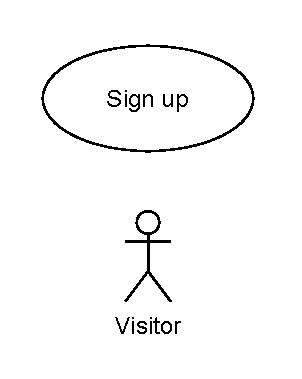
\includegraphics[width=0.3\linewidth]{drawio/visitor.pdf}
\end{frame}

% \begin{frame}
% \frametitle{Karting center administrator}

% \begin{table}
%     \tiny
%     \begin{tabular}{|p{2cm}|p{6cm}|}
%     \hline
%     Group name & \textbf{Karting center administrator} \\
%     \hline
%     Profile data & Name, Surname, e-mail address, password, address, phone number \\
%     \hline
%     Super group & Intranet \\
%     \hline
%     Sub group & None \\
%     \hline
%     Relevant use cases & CRUD on events, races, pilots, tracks, leaderboard, 
%     login, logout \\
%     \hline
%     Read & All \\
%     \hline
%     Write & All \\
%     \hline
%     \end{tabular}
%     \end{table}
% \end{frame}

% \begin{frame}
% \frametitle{Pilot}

% \begin{table}
%     \tiny
%     \begin{tabular}{|p{2cm}|p{6cm}|}
%     \hline
%     Group name & \textbf{Pilot} \\
%     \hline
%     Profile data & Name, Surname, e-mail address, password, address, phone number \\
%     \hline
%     Super group & Internet \\
%     \hline
%     Sub group & None \\
%     \hline
%     Relevant use cases & Create a race, Apply for an event, 
%     login, logout \\
%     \hline
%     Read & All \\
%     \hline
%     Write & Race, Leaderboard \\
%     \hline
%     \end{tabular}
%     \end{table}

% \end{frame}


% %%%%%%% DICTIONARY %%%%%%%

\section*{Data dictionary}

\subsection*{Primary entities}

\begin{frame}
\frametitle{Data dictionary}

% Table with two columns and 9 rows:
% - Name
% - Synonym
% - Description
% - Example of instance
% - Properties
% - Components
% - Relations
% - Superconcepts
% - Subconcepts

% table 9x2
\begin{table}
\tiny
\begin{tabular}{|p{2cm}|p{6cm}|}
\hline
Name & \textbf{Karting center} \\
\hline
Synonym & Go-karting center \\
\hline
Description & Karting center \\
\hline
Example of instance & 
Name: Mantova Karting Center \newline
\textit{City}: Mantova \newline
\textit{nPilots}: 5937 \newline
\textit{nRaces}: 12485 \newline
\textit{nEvents}:74 \newline
\textit{avgReviewScore}: 3.9 \\
\hline
Properties & 
Name: the name of the karting center\newline
\textit{City}: the city where the karting center is located\newline
\textit{nPilots}: the number of pilots that have raced in the karting center \newline
\textit{nRaces}: the number of races that took place in the karting center \newline
\textit{nEvents}: the number of events that had at least one race hosted by the karting center \newline
\textit{avgReviewScore}: the average score of the reviews of the karting center \\
\hline
Components & None \\
\hline
\end{tabular}
\end{table}

\end{frame}

\begin{frame}
\begin{table}
\tiny
\begin{tabular}{|p{2cm}|p{6cm}|}
\hline
Relations &
KartingCenter\_City (N:1): the city where the karting center is located \newline
KartingCenter\_KartingCenterAdmin (N:1): the karting center administrator of the karting center \newline
KartingCenter\_Clerk (1:N): the clerks of the karting center \newline
KartingCenter\_KartingCenterReview (1:N): the reviews of the karting center \newline
KartingCenter\_Track (1:N): the tracks of the karting center \newline
\textit{KartingCenter\_NPilotsRange} (N:1) the range within the number of pilots that have raced in the karting center falls \newline
\textit{KartingCenter\_NRacesRange} (N:1) the range within the number of races that took place in the karting center falls \newline
\textit{KartingCenter\_NEventsRange} (N:1) the range within the number of events that took place in the karting center falls \newline
\textit{KartingCenter\_ReviewScoreRange} (N:1) the range within the average score of the reviews of the karting center falls \newline
\textit{KartingCenter\_Event} (N:N) the events the karting center hosted \\
\hline
Superconcepts & None \\
\hline
Subconcepts & None \\
\hline
\end{tabular}
\end{table}
\end{frame}

\begin{frame}
\frametitle{City}
\begin{table}
\tiny
\begin{tabular}{|p{2cm}|p{6cm}|}
\hline
Name & \textbf{City} \\
\hline
Synonym & None \\
\hline
Description & City \\
\hline
Example of instance & 
Name: Mantova \\
\hline
Properties & 
Name: the name of the city \\
\hline
Components & None \\
\hline
Relations &
City\_KartingCenter (1:N): the karting centers located in the city \newline
\textit{City\_Track} (1:N): the tracks (inside a karting center) located in the city \newline
\textit{City\_Event} (N:N): the events that had at least one race on a track of a karting center
located in the city \\
\hline
Superconcepts & None \\
\hline
Subconcepts & None \\
\hline
\end{tabular}
\end{table}
\end{frame}

\begin{frame}
\frametitle{Track}
\begin{table}
\tiny
\begin{tabular}{|p{2cm}|p{6cm}|}
\hline
Name & \textbf{Track} \\
\hline
Synonym & Circuit \\
\hline
Description & Track \\
\hline
Example of instance &
Name: T1 \newline
Length: 700m \newline
\textit{City}: Mantova \newline
\textit{AsphaltType}: resin \newline
\textit{nRentalGoKarts}: 23 \newline
\textit{Difficulty}: Intermediate \newline
\textit{nPilots}: 3873 \newline
\textit{nRaces}: 7437 \newline
\textit{nEvents}: 43 \newline
\textit{avgReviewScore}: 4.2 \\
\hline
Properties &
Name: the name of the track \newline
Length: the length of the track \newline
\textit{City}: the city where the karting center the track belongs to is located \newline
\textit{AsphaltType}: the type of asphalt of the track \newline
\textit{nRentalGoKarts}: the number of rental go-karts available in the track \newline
\textit{Difficulty}: the difficulty of the track \newline
\textit{nPilots}: the number of pilots that have raced on the track \newline
\textit{nRaces}: the number of races that took place on the track \newline
\textit{nEvents}: the number of events that had at least one race on the track \newline
\textit{avgReviewScore}: the average score of the reviews of the track \\
\hline
Components & 
Timetable: the timetable of the track \newline
Leaderboard: a leaderboard of the track \\
\hline
\end{tabular}
\end{table}
\end{frame}

\begin{frame}
\begin{table}
\tiny
\begin{tabular}{|p{2cm}|p{6cm}|}
\hline
Relations &
Track\_KartingCenter (N:1): the karting center the track belongs to \newline
Track\_TrackReview (1:N): the reviews of the track \newline
Track\_Timetable (1:1): the timetable of the track \newline
Track\_Leaderboard (1:N): the leaderboards of the track \newline
Track\_Race (1:N): the races that took place on the track \newline
Track\_GoKart (1:N): the go-karts dedicated to the track \newline
Track\_GoKartModel (N:N): the go-kart models allowed on the track \newline
Track\_TrackAshpalt (N:1): the asphalt of the track \newline
Track\_TrackDifficulty (N:1): the difficulty of the track \newline
Track\_Pilot (N:N): the pilots that have the track as one of their favourite \newline
\textit{Track\_City} (N:1): the city where the karting center the track belongs to is located \newline
\textit{Track\_TrackLengthRange} (N:1): the range within the length of the track falls \newline
\textit{Track\_NPilotsRange} (N:1): the range within the number of pilots that have raced on the track falls \newline
\textit{Track\_NRacesRange} (N:1): the range within the number of races that took place on the track falls \newline
\textit{Track\_NEventsRange} (N:1): the range within the number of events that took place on the track falls \newline
\textit{Track\_ReviewScoreRange} (N:1): the range within the average score of the reviews of the track falls \\
\hline
Superconcepts & None \\
\hline
Subconcepts & 
PopularTrack: a track that is recurrent in the list of favourite tracks of pilots \\
\hline
\end{tabular}
\end{table}
\end{frame}

\begin{frame}
\frametitle{Go-kart}
\begin{table}
\tiny
\begin{tabular}{|p{2cm}|p{6cm}|}
\hline
Name & \textbf{Go-kart} \\
\hline
Synonym & Kart \\
\hline
Description & Go-kart \\
\hline
Example of instance &
Name: T1.1 \newline
GoKartModel: Sodi RX7 \\
\hline
Properties &
Name: the name of the go-kart \newline
\textit{GoKartModel}: the model of the go-kart \\
\hline
Components & None \\
\hline
Relations &
GoKart\_Track (N:1): the track the go-kart is dedicated to \newline
GoKart\_GoKartModel (N:1): the model of the go-kart \\
\hline
Superconcepts & None \\
\hline
Subconcepts & None \\
\hline
\end{tabular}
\end{table}
\end{frame}

\begin{frame}
\frametitle{Timetable}
\begin{table}
\tiny
\begin{tabular}{|p{2cm}|p{6cm}|}
\hline
Name & \textbf{Timetable} \\
\hline
Synonym & None \\
\hline
Description & Timetable \\
\hline
Example of instance &
\textit{TrackName}: T1 \\
\hline
Properties &
\textit{TrackName}: the name of the track \\
\hline
Components & None \\
\hline
Relations &
Timetable\_Track (1:1): the track the timetable belongs to \newline
Timetable\_Reservation (1:N): the reservations of the timetable \\
\hline
Superconcepts & None \\
\hline
Subconcepts & None \\
\hline
\end{tabular}
\end{table}
\end{frame}

\begin{frame}
\frametitle{Leaderboard}
\begin{table}
\tiny
\begin{tabular}{|p{2cm}|p{6cm}|}
\hline
Name & \textbf{Leaderboard} \\
\hline
Synonym & Ranking \\
\hline
Description & Leaderboard \\
\hline
Example of instance &
Title: Best of the week \newline
\textit{TrackName}: T1 \\
\hline
Properties &
Title: the title of the leaderboard \newline
\textit{TrackName}: the name of the track \\
\hline
Components & None \\
\hline
Relations &
Leaderboard\_Track (N:1): the track each leaderboard belongs to \newline
Leaderboard\_LapTime (N:N): the lap times the leaderboard focuses on \\
\hline
Superconcepts & None \\
\hline
Subconcepts & None \\
\hline
\end{tabular}
\end{table}
\end{frame}

\begin{frame}
\frametitle{Race}
\begin{table}
\tiny
\begin{tabular}{|p{2cm}|p{6cm}|}
\hline
Name & \textbf{Race} \\
\hline
Synonym & None \\
\hline
Description & Race \\
\hline
Example of instance &
ID: 2036 \newline
Date: 2024-02-15 \newline
Start: 15:00 \newline
End: 15:09 \newline
ForEvent: false \newline
\textit{GoKartingCenterName}: Mantova Karting Center \newline
\textit{TrackName}: T1 \newline
\textit{nPartecipants}: 8 \newline
\textit{fastestLapTime}: 00:00:48.595 \\
\hline
Properties &
ID \newline
Date \newline
Start \newline
End \newline
ForEvent: whether the race was created by an organizer for an event or not \newline
\textit{GoKartingCenterName} \newline
\textit{TrackName}: the name of the track that hosts the race \newline
\textit{nPartecipants} \newline
\textit{fastestLapTime} \\
\hline
Components & Reservation \\
\hline
\end{tabular}
\end{table}
\end{frame}

\begin{frame}
\begin{table}
\tiny
\begin{tabular}{|p{2cm}|p{6cm}|}
\hline
Relations & 
Race\_Track (N:1): the track the race has been raced on \newline
Race\_Reservation (1:1): the reservation that has been made for the race \newline
Race\_Pilot (N:N): the pilots that participated in the race \newline
Race\_LapTime (1:N): every lap-time of every pilot that participated in the race \newline
Race\_Event (N:1): the event the race is part of \newline
\textit{Race\_Pilot} (1:N): the pilots who have this race as their last race \newline
\textit{Race\_Laptime} (1:1): the best lap-time of the race \\
\hline
Superconcepts & None \\
\hline
Subconcepts & None \\
\hline
\end{tabular}
\end{table}
\end{frame}

\begin{frame}
\frametitle{Reservation}
\begin{table}
\tiny
\begin{tabular}{|p{2cm}|p{6cm}|}
\hline
Name & \textbf{Reservation} \\
\hline
Synonym & Booking \\
\hline
Description & Reservation \\
\hline
Example of instance &
Date: 2024-02-15 \newline
Start: 15:00 \newline
End: 15:09 \newline
\textit{ReservedByPilot}: denisfesta \newline
\textit{ReservedByOrganizer}: None \newline
\textit{ConfirmedByClerk}: Jessica \\
\hline
Properties &
Date \newline
Start \newline
End \newline
\textit{ReservedByPilot}: the pilot who made the reservation (this property 
is mutually exclusive with \textit{ReservedByOrganizer}) \newline
\textit{ReservedByOrganizer}: the organizer who made the reservation (this property
is mutually exclusive with \textit{ReservedByPilot}) \newline
\textit{ConfirmedByClerk}: the clerk who confirmed the reservation \\
\hline
Components & None \\
\hline
Relations &
Reservation\_Timetable (N:1): the timetable where the reservation is stored \newline
Reservation\_Pilot (N:1): the pilot who made the reservation \newline
Reservation\_Organizer (N:1): the organizer who made the reservation \newline
Reservation\_Clerk (N:1): the clerk who confirmed the reservation \newline
Reservation\_Race (1:1): the race this reservation has been made for \\
\hline
Superconcepts & None \\
\hline
Subconcepts & None \\
\hline
\end{tabular}
\end{table}
\end{frame}

\begin{frame}
\frametitle{Lap-time}
\begin{table}
\tiny
\begin{tabular}{|p{2cm}|p{6cm}|}
\hline
Name & \textbf{Lap-time} \\
\hline
Synonym & Lap \\
\hline
Description & Lap-time \\
\hline
Example of instance &
LapNumber: 7 \newline
LapTime: 00:00:48.595 \\
\hline
Properties &
LapNumber: the \textit{LapNumber}-th lap \newline
LapTime: the time measured for the \textit{LapNumber}-th lap for 
a particular pilot \\
\hline
Components & None \\
\hline
Relations & 
LapTime\_Pilot (N:1): the pilot who made the lap-time \newline
LapTime\_Race (N:1): the race where the lap-time has been made \newline
\textit{LapTime\_Race} (1:1): in case the lap-time is the best of a race \newline
\textit{LapTime\_Leaderboard} (N:N): the leaderboards where the lap-time is displayed \\
\hline
Superconcepts & None \\
\hline
Subconcepts & None \\
\hline
\end{tabular}
\end{table}
\end{frame}

\begin{frame}
\frametitle{Data dictionary}
\begin{table}
\tiny
\begin{tabular}{|p{2cm}|p{6cm}|}
\hline
Name & \textbf{Application} \\
\hline
Synonym & Request \\
\hline
Description & Application \\
\hline
Example of instance &
Confirmed: true \newline
\textit{EventName}: Mantova Karting Cup 2024 \newline
\textit{RequestFromPilot}: denisfesta \\
\hline
Properties &
Confirmed: whether the application has been confirmed or not (the organizer who
created the event is the
only one who can accept an application) \newline
\textit{EventName}: the name of the event the application has been made for \newline
\textit{RequestFromPilot}: the pilot who made the application \\
\hline
Components & None \\
\hline
Relations &
Application\_Pilot (N:1): the pilot who made the application \newline
Application\_Event (N:1): the event the application has been made for \\
\hline
Superconcepts & None \\
\hline
Subconcepts & None \\
\hline
\end{tabular}
\end{table}
\end{frame}

\begin{frame}
\frametitle{Data dictionary}
\begin{table}
\tiny
\begin{tabular}{|p{2cm}|p{6cm}|}
\hline
Name & \textbf{Event} \\
\hline
Synonym & Tournament \\
\hline
Description & Event \\
\hline
Example of instance &
Name: Mantova Karting Cup 2024 \newline
Price: 100 \newline
\textit{FirstDate}: 2024-02-15 \newline
\textit{OrganizerName}: WD40 \newline
\textit{EventCategory}: Open \newline
\textit{nPartecipants}: 64 \newline
\textit{nRaces}: 12 \newline
\textit{nReviews}: 23 \newline
\textit{avgReviewScore}: 4.5 \\
\hline
Properties &
Name: the name of the event \newline
Price: the price of the event \newline
\textit{FirstDate}: the date of the first race of the event \newline
\textit{OrganizerName}: the username of the organizer who created the event \newline
\textit{EventCategory}: the category of the event (\textit{open, intermediate, pro})\newline
\textit{nPartecipants}: the number of pilots who applied for the event and whose application was confirmed\newline
\textit{nRaces}: the number of races of the event \newline
\textit{nReviews}: the number of written reviews about the event \newline
\textit{avgReviewScore}: the average score of the reviews about the event \\
\hline
Components & None \\
\hline
\end{tabular}
\end{table}
\end{frame}

\begin{frame}
\begin{table}
\tiny
\begin{tabular}{|p{2cm}|p{6cm}|}
\hline
Relations &
Event\_Organizer (N:1): the organizer who created the event \newline
Event\_Application (1:N): the applications received for the event \newline
Event\_Race (1:N): the races of the event \newline
Event\_EventCategory (N:1): the category of the event \newline
Event\_EventReview (1:N): the reviews about the event \newline
\textit{Event\_ReviewScoreRange} (N:1): the range within the average score of the reviews about the event falls \newline
\textit{Event\_Pilot} (N:N): the pilots who applied for the event and whose application was confirmed \newline
\textit{Event\_PriceRange} (N:1): the range within the price of the event falls \newline
\textit{Event\_City} (N:N): the cities where the races of the event took place \newline
\textit{Event\_Track} (N:N): the tracks that hosted the races of the event \newline
\textit{Event\_KartingCenter} (N:N): the karting centers whose tracks hosted the races of the event \\
\hline
Superconcepts & None \\
\hline
Subconcepts & Controversial event, Popular evenet, Upcoming event \\
\hline
\end{tabular}
\end{table}
\end{frame}

\begin{frame}
    \frametitle{Data dictionary}
    \begin{table}
    \tiny
    \begin{tabular}{|p{2cm}|p{6cm}|}
    \hline
    Name & \textbf{Review} \\
    \hline
    Synonym & Opinion \\
    \hline
    Description & Review \\
    \hline
    Example of instance &
    TextReview: Fantastic track, with a lot of bumps and holes. \newline
    Score: 4/5 \\
    \hline
    Properties &
    TextReview: the text of the review \newline
    Score: the score of the review \\
    \hline
    Components & None \\
    \hline
    Relations & None \\
    \hline
    Superconcepts & None \\
    \hline
    Subconcepts & KartingCenterReview, TrackReview, EventReview \\
    \hline
    \end{tabular}
    \end{table}
\end{frame}

\begin{frame}
    \frametitle{Data dictionary}
    \begin{table}
    \tiny
    \begin{tabular}{|p{2cm}|p{6cm}|}
    \hline
    Name & \textbf{KartingCenterReview} \\
    \hline
    Synonym & None \\
    \hline
    Description & Karting center review \\
    \hline
    Example of instance &
    TextReview (inherited from \textbf{Review}): Very rude and violent staff, but nice tracks! \newline
    Score (inherited from \textbf{Review}): 4/5 \\
    \hline
    Properties & None \\
    \hline
    Components & None \\
    \hline
    Relations &
    KartingCenterReview\_KartingCenter (N:1): the karting center the review is about \newline
    KartingCenterReview\_Pilot (N:1): the pilot who wrote the review \\
    \hline
    Superconcepts & Review \\
    \hline
    Subconcepts & None \\
    \hline
    \end{tabular}
    \end{table}
\end{frame}

\begin{frame}
    \frametitle{Data dictionary}
    \begin{table}
    \tiny
    \begin{tabular}{|p{2cm}|p{6cm}|}
    \hline
    Name & \textbf{TrackReview} \\
    \hline
    Synonym & None \\
    \hline
    Description & Track review \\
    \hline
    Example of instance &
    TextReview (inherited from \textbf{Review}): The track is very nice, but the asphalt is not in good conditions. \newline
    Score (inherited from \textbf{Review}): 3/5 \\
    \hline
    Properties & None \\
    \hline
    Components & None \\
    \hline
    Relations &
    TrackReview\_Track (N:1): the track the review is about \newline
    TrackReview\_Pilot (N:1): the pilot who wrote the review \\
    \hline
    Superconcepts & Review \\
    \hline
    Subconcepts & None \\
    \hline
    \end{tabular}
    \end{table}
\end{frame}

\begin{frame}
    \frametitle{Data dictionary}
    \begin{table}
    \tiny
    \begin{tabular}{|p{2cm}|p{6cm}|}
    \hline
    Name & \textbf{EventReview} \\
    \hline
    Synonym & None \\
    \hline
    Description & Event review \\
    \hline
    Example of instance &
    TextReview (inherited from \textbf{Review}): The event was a mess, delayed a couple of times and 
    some pilots were not correctly registered. \newline
    Score (inherited from \textbf{Review}): 2/5 \\
    \hline
    Properties & None \\
    \hline
    Components & None \\
    \hline
    Relations &
    EventReview\_Event (N:1): the event the review is about \newline
    EventReview\_Pilot (N:1): the pilot who wrote the review \\
    \hline
    Superconcepts & Review \\
    \hline
    Subconcepts & None \\
    \hline
    \end{tabular}
    \end{table}
\end{frame}

\subsection*{Users' entities}

\begin{frame}
    \frametitle{Data dictionary}
    \begin{table}
    \tiny
    \begin{tabular}{|p{2cm}|p{6cm}|}
    \hline
    Name & \textbf{User} \\
    \hline
    Synonym & None \\
    \hline
    Description & User \\
    \hline
    Example of instance &
    Username: denisfesta \newline
    Password: 12345asdf!  \newline
    Email: d.festa004@studenti.unibs.it \newline
    Name: Denis \newline
    Surname: Festa \newline
    Address: Via Trento 5, Rovato (BS) \\
    \hline
    Properties &
    Username: the username of the user \newline
    Password: the password of the user \newline
    Email: the email address of the user \newline
    Name: the name of the user \newline
    Surname: the surname of the user \newline
    Address: the address of the user \\
    \hline
    Components & None \\
    \hline
    Relations & None \\
    \hline
    Superconcepts & None \\
    \hline
    Subconcepts & Admin, KartingCenterAdmin, Clerk, Organizer, Pilot \\
    \hline
    \end{tabular}
    \end{table}
\end{frame}

\begin{frame}
    \frametitle{Data dictionary}
    \begin{table}
    \tiny
    \begin{tabular}{|p{2cm}|p{6cm}|}
    \hline
    Name & \textbf{Admin} \\
    \hline
    Synonym & Administrator \\
    \hline
    Description & The administrator does not have any relation with other 
    entities of the information system but is needed to create karting center administrators,
    organizers and all the auxiliary objects useful for the visitor to explore easily. \\
    \hline
    Example of instance & Empty (all the properties are inherited from \textbf{User}) \\
    \hline
    Properties & None \\
    \hline
    Components & None \\
    \hline
    Relations & None \\
    \hline
    Superconcepts & User \\
    \hline
    Subconcepts & None \\
    \hline
    \end{tabular}
    \end{table}
\end{frame}

\begin{frame}
    \frametitle{Data dictionary}
    \begin{table}
    \tiny
    \begin{tabular}{|p{2cm}|p{6cm}|}
    \hline
    Name & \textbf{KartingCenterAdmin} \\
    \hline
    Synonym & None \\
    \hline
    Description & Karting center administrator \\
    \hline
    Example of instance & Empty (all the properties are inherited from \textbf{User}) \\
    \hline
    Properties & None \\
    \hline
    Components & None \\
    \hline
    Relations &
    KartingCenterAdmin\_KartingCenter (1:N): the karting centers the administrator is in charge of \\
    \hline
    Superconcepts & User \\
    \hline
    Subconcepts & None \\
    \hline
    \end{tabular}
    \end{table}
\end{frame}

\begin{frame}
    \frametitle{Data dictionary}
    \begin{table}
    \tiny
    \begin{tabular}{|p{2cm}|p{6cm}|}
    \hline
    Name & \textbf{Clerk} \\
    \hline
    Synonym & None \\
    \hline
    Description & Clerk \\
    \hline
    Example of instance & Empty (all the properties are inherited from \textbf{User}) \\
    \hline
    Properties & None \\
    \hline
    Components & None \\
    \hline
    Relations &
    Clerk\_KartingCenter (N:1): the karting center the clerk works for \newline
    Clerk\_Reservation (1:N): the reservations the clerk confirmed \\
    \hline
    Superconcepts & User \\
    \hline
    Subconcepts & None \\
    \hline
    \end{tabular}
    \end{table}
\end{frame}

\begin{frame}
    \frametitle{Data dictionary}
    \begin{table}
    \tiny
    \begin{tabular}{|p{2cm}|p{6cm}|}
    \hline
    Name & \textbf{Organizer} \\
    \hline
    Synonym & None \\
    \hline
    Description & Organizer \\
    \hline
    Example of instance & Empty (all the properties are inherited from \textbf{User}) \\
    \hline
    Properties & None \\
    \hline
    Components & None \\
    \hline
    Relations &
    Organizer\_Event (1:N): the events the organizer created \newline
    Organizer\_Reservation (1:N): the reservations the organizer requested \\
    \hline
    Superconcepts & User \\
    \hline
    Subconcepts & None \\
    \hline
    \end{tabular}
    \end{table}
\end{frame}


\begin{frame}
    \frametitle{Data dictionary}
    \begin{table}
    \tiny
    \begin{tabular}{|p{2cm}|p{6cm}|}
    \hline
    Name & \textbf{Pilot} \\
    \hline
    Synonym & None \\
    \hline
    Description & Pilot \\
    \hline
    Example of instance &
    Username (inherited from \textbf{User}): denisfesta \newline
    Password (inherited from \textbf{User}): 12345asdf!  \newline
    Email (inherited from \textbf{User}): d.festa004@studenti.unibs.it \newline
    Name (inherited from \textbf{User}): Denis \newline
    Surname (inherited from \textbf{User}): Festa \newline
    Address (inherited from \textbf{User}): Via Trento 5, Rovato (BS) \newline
    Age: 25 \newline
    Weight: 70 \\
    \hline
    Properties &
    Age: the age of the pilot \newline
    Weight: the weight of the pilot \\
    \hline
    Components & None \\
    \hline
    Relations &
    Pilot\_KartingCenterReview (1:N): the reviews the pilot wrote about karting centers \newline
    Pilot\_TrackReview (1:N): the reviews the pilot wrote about tracks \newline
    Pilot\_EventReview (1:N): the reviews the pilot wrote about events \newline
    Pilot\_Application (1:N): the applications the pilot made \newline
    Pilot\_Reservation (1:N): the reservations the pilot made \newline
    Pilot\_Track (N:N): the tracks the pilot has as favorite \newline
    Pilot\_Race (N:N): the races the pilot participated in \newline
    Pilot\_LapTime (1:N): the lap-times the pilot made \newline
    \textit{Pilot\_Race} (N:1): the last race the pilot participated in \newline
    \textit{Pilot\_Event} (N:N): the events the pilot was accepted to participate in \\
    \hline
    Superconcepts & User \\
    \hline
    Subconcepts & None \\
    \hline
    \end{tabular}
    \end{table}
\end{frame}

\subsection*{Auxiliary entities}

\begin{frame}
    \frametitle{Data dictionary}
    \begin{table}
    \tiny
    \begin{tabular}{|p{2cm}|p{6cm}|}
    \hline
    Name & \textbf{ReviewScoreRange} \\
    \hline
    Synonym & None \\
    \hline
    Description & Review score range \\
    \hline
    Example of instance &
    LowerBoundIncluded: 1 \newline
    UpperBoundExcluded: 3 \\
    \hline
    Properties &
    LowerBoundIncluded: the lower bound of the range \newline
    UpperBoundExcluded: the upper bound of the range \\
    \hline
    Components & None \\
    \hline
    Relations &
    ReviewScoreRange\_KartingCenter (1:N): the karting centers whose average review score falls in the range \newline
    ReviewScoreRange\_Track (1:N): the tracks whose average review score falls in the range \newline
    ReviewScoreRange\_Event (1:N): the events whose average review score falls in the range \\
    \hline
    Superconcepts & None \\
    \hline
    Subconcepts & None \\
    \hline
    \end{tabular}
    \end{table}
\end{frame}

\begin{frame}
    \frametitle{Data dictionary}
    \begin{table}
    \tiny
    \begin{tabular}{|p{2cm}|p{6cm}|}
    \hline
    Name & \textbf{NPilotsRange} \\
    \hline
    Synonym & None \\
    \hline
    Description & A range of number of pilots \\
    \hline
    Example of instance &
    LowerBoundIncluded: 0 \newline
    UpperBoundExcluded: 100 \\
    \hline
    Properties &
    LowerBoundIncluded: the lower bound of the range \newline
    UpperBoundExcluded: the upper bound of the range \\
    \hline
    Components & None \\
    \hline
    Relations &
    NPilotsRange\_KartingCenter (1:N): the karting centers whose number of pilots falls in the range \newline
    NPilotsRange\_Track (1:N): the tracks whose number of pilots falls in the range \\
    \hline
    Superconcepts & None \\
    \hline
    Subconcepts & None \\
    \hline
    \end{tabular}
    \end{table}
\end{frame}

\begin{frame}
    \frametitle{Data dictionary}
    \begin{table}
    \tiny
    \begin{tabular}{|p{2cm}|p{6cm}|}
    \hline
    Name & \textbf{NRacesRange} \\
    \hline
    Synonym & None \\
    \hline
    Description & A range of number of races \\
    \hline
    Example of instance &
    LowerBoundIncluded: 10000 \newline
    UpperBoundExcluded: 20000 \\
    \hline
    Properties &
    LowerBoundIncluded: the lower bound of the range \newline
    UpperBoundExcluded: the upper bound of the range \\
    \hline
    Components & None \\
    \hline
    Relations &
    NRacesRange\_KartingCenter (1:N): the karting centers whose number of races 
    (the sum of all the races on all the tracks of that karting center) falls in the range \newline
    NRacesRange\_Track (1:N): the tracks whose number of races that took place on them falls in the range \\
    \hline
    Superconcepts & None \\
    \hline
    Subconcepts & None \\
    \hline
    \end{tabular}
    \end{table}
\end{frame}

\begin{frame}
    \frametitle{Data dictionary}
    \begin{table}
    \tiny
    \begin{tabular}{|p{2cm}|p{6cm}|}
    \hline
    Name & \textbf{NEventsRange} \\
    \hline
    Synonym & None \\
    \hline
    Description & A range of number of events \\
    \hline
    Example of instance &
    LowerBoundIncluded: 0 \newline
    UpperBoundExcluded: 10 \\
    \hline
    Properties &
    LowerBoundIncluded: the lower bound of the range \newline
    UpperBoundExcluded: the upper bound of the range \\
    \hline
    Components & None \\
    \hline
    Relations &
    NEventsRange\_KartingCenter (1:N): the karting centers whose number of hosted events falls in the range \newline
    NEventsRange\_Track (1:N): the tracks whose number of events that took place on them falls in the range \\
    \hline
    Superconcepts & None \\
    \hline
    Subconcepts & None \\
    \hline
    \end{tabular}
    \end{table}
\end{frame}

\begin{frame}
    \frametitle{Data dictionary}
    \begin{table}
    \tiny
    \begin{tabular}{|p{2cm}|p{6cm}|}
    \hline
    Name & \textbf{GoKartModel} \\
    \hline
    Synonym & None \\
    \hline
    Description & Go-kart model \\
    \hline
    Example of instance &
    GoKartModel: Sodi RX7 \\
    \hline
    Properties &
    GoKartModel: the name of the go-kart model \\
    \hline
    Components & None \\
    \hline
    Relations &
    GoKartModel\_GoKart (1:N): the go-karts of that model \newline
    GoKartModel\_Track (N:N): the tracks where that model is available\\
    \hline
    Superconcepts & None \\
    \hline
    Subconcepts & None \\
    \hline
    \end{tabular}
    \end{table}
\end{frame}


\begin{frame}
    \frametitle{Data dictionary}
    \begin{table}
    \tiny
    \begin{tabular}{|p{2cm}|p{6cm}|}
    \hline
    Name & \textbf{TrackAsphalt} \\
    \hline
    Synonym & None \\
    \hline
    Description & Track asphalt \\
    \hline
    Example of instance &
    TrackAsphalt: Asphalt \\
    \hline
    Properties &
    TrackAsphalt: the name of the track asphalt \\
    \hline
    Components & None \\
    \hline
    Relations &
    TrackAsphalt\_Track (1:N): the tracks with that asphalt \\
    \hline
    Superconcepts & None \\
    \hline
    Subconcepts & None \\
    \hline
    \end{tabular}
    \end{table}
\end{frame}


\begin{frame}
    \frametitle{Data dictionary}
    \begin{table}
    \tiny
    \begin{tabular}{|p{2cm}|p{6cm}|}
    \hline
    Name & \textbf{TrackDifficulty} \\
    \hline
    Synonym & None \\
    \hline
    Description & Track difficulty \\
    \hline
    Example of instance &
    TrackDifficulty: Intermediate \\
    \hline
    Properties &
    TrackDifficulty: the name of the track difficulty \\
    \hline
    Components & None \\
    \hline
    Relations &
    TrackDifficulty\_Track (1:N): the tracks with that difficulty \\
    \hline
    Superconcepts & None \\
    \hline
    Subconcepts & None \\
    \hline
    \end{tabular}
    \end{table}
\end{frame}


\begin{frame}
    \frametitle{Data dictionary}
    \begin{table}
    \tiny
    \begin{tabular}{|p{2cm}|p{6cm}|}
    \hline
    Name & \textbf{TrackLengthRange} \\
    \hline
    Synonym & None \\
    \hline
    Description & Track length range \\
    \hline
    Example of instance &
    LowerBoundIncluded: 0 \newline
    UpperBoundExcluded: 300 \\
    \hline
    Properties &
    LowerBoundIncluded: the lower bound of the range \newline
    UpperBoundExcluded: the upper bound of the range \\
    \hline
    Components & None \\
    \hline
    Relations &
    TrackLengthRange\_Track (1:N): the tracks whose length falls in the range \\
    \hline
    Superconcepts & None \\
    \hline
    Subconcepts & None \\
    \hline
    \end{tabular}
    \end{table}
\end{frame}


\begin{frame}
    \frametitle{Data dictionary}
    \begin{table}
    \tiny
    \begin{tabular}{|p{2cm}|p{6cm}|}
    \hline
    Name & \textbf{PopularTrack} \\
    \hline
    Synonym & None \\
    \hline
    Description & A popular track is a track that has been selected as favorite by
    at least $N$ pilots.\newline
    This subclass of \textbf{Track} is to be considered as a \textbf{view} of the database
    that invites the visitor during its navigation and at the same time speeds up the
    execution of the query. \\
    \hline
    Example of instance & Empty (all the properties are inherited from \textbf{Track}) \\
    \hline
    Properties & None \\
    \hline
    Components & None \\
    \hline
    Relations & None \\
    \hline
    Superconcepts & Track \\
    \hline
    Subconcepts & None \\
    \hline
    \end{tabular}
    \end{table}
\end{frame}


\begin{frame}
    \frametitle{Data dictionary}
    \begin{table}
    \tiny
    \begin{tabular}{|p{2cm}|p{6cm}|}
    \hline
    Name & \textbf{ControversialEvent} \\
    \hline
    Synonym & None \\
    \hline
    Description & A controversial event is an event that has received at least $N$ reviews
    with a score lower than 25\% of the maximum score and at least $N$ reviews 
    with a score higher than 75\% of the maximum score.\newline
    This subclass of \textbf{Event} is to be considered as a \textbf{view} of the database. \\
    \hline
    Example of instance & Empty (all the properties are inherited from \textbf{Event}) \\
    \hline
    Properties & None \\
    \hline
    Components & None \\
    \hline
    Relations & None \\
    \hline
    Superconcepts & Event \\
    \hline
    Subconcepts & None \\
    \hline
    \end{tabular}
    \end{table}
\end{frame}


\begin{frame}
    \frametitle{Data dictionary}
    \begin{table}
    \tiny
    \begin{tabular}{|p{2cm}|p{6cm}|}
    \hline
    Name & \textbf{PopularEvent} \\
    \hline
    Synonym & None \\
    \hline
    Description & A popular event is an event that already took place, 
    to which at least $N$ pilots partecipated 
    and that received at least $N$ reviews. \newline
    This subclass of \textbf{Event} is to be considered as a \textbf{view} of the database. \\
    \hline
    Example of instance & Empty (all the properties are inherited from \textbf{Event}) \\
    \hline
    Properties & None \\
    \hline
    Components & None \\
    \hline
    Relations & None \\
    \hline
    Superconcepts & Event \\
    \hline
    Subconcepts & None \\
    \hline
    \end{tabular}
    \end{table}
\end{frame}


\begin{frame}
    \frametitle{Data dictionary}
    \begin{table}
    \tiny
    \begin{tabular}{|p{2cm}|p{6cm}|}
    \hline
    Name & \textbf{UpcomingEvent} \\
    \hline
    Synonym & None \\
    \hline
    Description & An upcoming event is an 
    event that has not yet taken place, its attribute \textit{FirstDate} is in the future. \newline
    This subclass of \textbf{Event} is to be considered 
    as a \textbf{view} of the database. \\
    \hline
    Example of instance & Empty (all the properties are inherited from \textbf{Event}) \\
    \hline
    Properties & None \\
    \hline
    Components & None \\
    \hline
    Relations & None \\
    \hline
    Superconcepts & Event \\
    \hline
    Subconcepts & None \\
    \hline
    \end{tabular}
    \end{table}
\end{frame}


\begin{frame}
    \frametitle{Data dictionary}
    \begin{table}
    \tiny
    \begin{tabular}{|p{2cm}|p{6cm}|}
    \hline
    Name & \textbf{PriceRange}  \\
    \hline
    Synonym & None \\
    \hline
    Description & A range of price of the events \\
    \hline
    Example of instance &
    LowerBoundIncluded: 0 \newline
    UpperBoundExcluded: 50 \\
    \hline
    Properties &
    LowerBoundIncluded: the lower bound of the range \newline
    UpperBoundExcluded: the upper bound of the range \\
    \hline
    Components & None \\
    \hline
    Relations &
    PriceRange\_Event (1:N): the events whose price falls in the range \\
    \hline
    Superconcepts & None \\
    \hline
    Subconcepts & None \\
    \hline
    \end{tabular}
    \end{table}
\end{frame}


\begin{frame}
    \frametitle{Data dictionary}
    \begin{table}
    \tiny
    \begin{tabular}{|p{2cm}|p{6cm}|}
    \hline
    Name & \textbf{EventCategory} \\
    \hline
    Synonym & None \\
    \hline
    Description & The event can be open to every pilot (entry level difficulty),
    intermediate (for those pilots that feel more competitive) and 
    pro (only pilots that show up at a high rank in the leaderboards can participate). \\
    \hline
    Example of instance &
    EventCategory: Open \\
    \hline
    Properties &
    EventCategory: the name of the event category \\
    \hline
    Components & None \\
    \hline
    Relations &
    EventCategory\_Event (1:N): the events with that category \\
    \hline
    Superconcepts & None \\
    \hline
    Subconcepts & None \\
    \hline
    \end{tabular}
    \end{table}
\end{frame}


























% Quando voglio visitare un nuovo arrivo
% utilizzo non una query ma una derivata
% che calcola la query una volta sola

\end{document}